\documentclass[titlepage]{article}

\usepackage[italian]{babel}
\usepackage[OT1]{fontenc}
\usepackage{cmbright}
\usepackage{csquotes}
\usepackage{amsmath}
\usepackage{fancyhdr}
\usepackage{amssymb}
\usepackage{tikz}
\usepackage{subcaption}
\usepackage{amsthm}
\usepackage{xurl}
\usepackage{multirow}
\usepackage{enumitem}
\usepackage[hidelinks]{hyperref}
\usepackage[backend=biber, style=authoryear-comp, maxcitenames=2]{biblatex}

% document ----------------------------

\addbibresource{ref.bib}

\begin{document}

\begin{titlepage}
  \center % Center everything on the page

  %----------------------------------------------------------------------------------------
  %	HEADING SECTIONS
  %----------------------------------------------------------------------------------------

  \begingroup
  \noindent
  \begin{minipage}[t]{0.16\textwidth}
    \vspace{-5mm}{
\includegraphics[width=\textwidth]{images/logo.png}}
  \end{minipage}%
  \hfill
  \begin{minipage}[t]{0.8\textwidth}\raggedright
    {\large Università degli Studi di Milano Bicocca} \\
    \textbf{Scuola di Scienze} \\
    \textbf{Dipartimento di Informatica, Sistemistica e Comunicazione} \\
    \textbf{Corso di laurea magistrale in Informatica} \\
  \end{minipage}%
  \par\endgroup

  %----------------------------------------------------------------------------------------
  %	TITLE SECTION
  %----------------------------------------------------------------------------------------

  \vfill
  {\Large Sistemi Complessi: Modelli e Simulazione}\\[1cm]
  {\LARGE\bfseries Tsunami Evacuation Simulation}\\[0.4cm]
  \vfill

  %----------------------------------------------------------------------------------------
  %	AUTHOR SECTION
  %----------------------------------------------------------------------------------------

  \large
  Giuseppe Magazzù \\
  Gaetano Magazzù \\[1cm]

  %----------------------------------------------------------------------------------------
  %	DATE SECTION
  %----------------------------------------------------------------------------------------

  {\large A.A. 2021 - 2022}\\[2cm]

  %----------------------------------------------------------------------------------------
\end{titlepage}


\pagenumbering{roman}

\tableofcontents

%\clearpage
\pagenumbering{arabic}


\section{Introduzione}
Gli tsunami sono eventi naturali pericolosi che negli ultimi decenni 
hanno causato la morte di oltre 250.000 persone e si verificano spesso 
dopo un terremoto.

Rispetto agli altri eventi naturali come uragani, eruzioni vulcaniche e inondazioni, 
i tempi di allerta sono molto più brevi \parencite{katada2006integrated}.
%
Infatti possono raggiungere la costa dopo 20-40 minuti dalla prima scossa oppure dopo ore.
Nel primo caso si parla di near-field tsunami, mentre nel secondo di far-field tsunami. 

Considerando le disastrose conseguenze dovute a questi fenomeni è necessaria un'evacuazione efficiente per salvare vite umane. 

Simulare un'evacuazione in caso di tsunami rappresenta uno strumento molto utile per 
prendere delle contromisure e migliorare le modalità di evacuazione.

I modelli agent-based sono ideali per gestire uno scenario complesso come quello di un'evacuazione da tsunami e
per modellare le diverse dinamiche che emergono quando diversi individui interagiscono tra loro durante un'emergenza. 

Molti modelli non considerano o semplificano alcuni fattori importanti nell'evacuazione da tsunami.
Alcuni modelli limitano i pedoni a muoversi solo lungo la strada e non permettono di sfruttare le aree aperte. 
Altri non gestiscono o riducono in parte le interazioni tra pedoni e altri veicoli nel caso di un'evacuazione multimodale.
%
Spesso non vengono considerati i danni causati dal terremoto prima o durante l'evacuazione.

L'obiettivo di questo lavoro è sviluppare un modello di evacuazione multi-agente in caso di tsunami
di auto e pedoni e gestire le interazioni tra gli agenti, 
in particolare nelle intersezioni.
%
Il modello è stato sviluppato usando come base di partenza quello di \textcite{mostafizi2019agent}.

Nella sezione \ref{sec:background} vengono presentati gli elementi principali di un modello di evacuzione da tsunami.
Nella sezione \ref{sec:stato-arte} viene riportato lo stato dell'arte.
%
Nelle sezioni \ref{sec:modello} e \ref{sec:estensione} viene descritto il modello base e la sua estensione e 
nelle sezioni \ref{sec:simulazione} e \ref{sec:analisi} viene mostrata l'impostazione della simulazione e 
l'analisi dei risultati.
%
Infine la conclusione nella sezione \ref{sec:conclusione}.

\pagebreak

\section{Background}
\# TODO: descrivere le componenti di un modello generico di simulazione di evacuazione in caso di tsunami..

\subsection{Elementi del Modello}

\subsubsection{Popolazione}
Distribuzione... 

\subsubsection{Rete stradale}

\subsubsection{Rifugi}
luoghi sicuri dove evacuare. possono essere orizzontali o verticali

\subsubsection{Inondazione dello tsunami}
(time-dependent) scenarios, casualties (wave height Hc) 

\subsection{Evacuazione}
Milling Time....

L'evacuazione può avvenire in due modi: a piedi e in auto. Una volta che ogni agente decide
in che modo evacuare non cambierà scelta per tutta la simulazione.

All'inizio della simulazione ogni agente decide come destinazione il rifugio più vicino 
che verrà raggiunto seguendo il percorso più breve (\it{shortest path}).


\subsubsection{Movimento dei Pedoni}
- descrizione stato dell agente (la propria visione dell ambiente)

- velocità costante di [valore]

Each pedestrian agent is assigned a
walking speed which will not vary over the simulation

The effect of tiredness of evacuees and topography of the
environment have been neglected in this simulation

All evacuees begin to evacuate by
foot to the nearest road.

\subsubsection{Movimento delle Auto}
- descrizione stato dell agente (la propria visione dell ambiente)

- descrizione car following model

\subsection{Limitazioni}

tutte le strade a senso unico con un unica corsia
con limite massimo di velocità di 30mph

non vengono gestite interazioni tra macchine e pedoni.

l'accesso ad un link / le intersezioni non sono gestite.

Nel lavoro [] vengono menzionati turisti e residenti
ma i turisti non vengono gestiti veramente è trattati
con una stessa entità senza un comportamento differenziato.

\section{Stato dell'Arte}
\label{sec:stato-arte}
In questa sezione verrà descritto lo stato dell'arte dei modelli \textit{agent-based} di evacuazione da tsunami, senza focalizzarsi sui modelli di inondazione.
Successivamente alcuni lavori verranno approfonditi nelle sottosezioni seguenti, in particolare modelli \textit{network-based} con scenari multimodali.

I primi modelli di evacuazione da tsunami sono stati basati sui modelli \textit{network-based} utilizzati per l'evacuazione da altri disastri come
uragani, incendi e inondazioni \parencite{usuzawa1997development, imamura2001development}.

Uno dei primi aspetti che è stato preso in considerazione è il comportamento umano,
in particolare le reazioni dei residenti all'arrivo dello tsunami
e il tempo che ci mettono per iniziare a evacuare.

Queste informazioni sono state raccolte tramite dei questionari rivolti ai residenti
e usate per stimare i tempi di partenza dell'evacuazione \parencite{imamura2001development, saito2004simulation}.

Questi primi modelli \textit{network-based} hanno usato come regola di \textit{path finding}
proseguire verso il nodo con altitudine maggiore.
Successivamente si è passati a usare il percorso
più breve \parencite{katada2004disaster} e altre strategie di routing basate sull'apprendimento 
come Nash equilibrium e system optimal \parencite{lammel2009towards}.

Un altro aspetto importante per l'evacuazione è la conoscenza dell'ambiente da parte degli agenti.
Alcuni lavori hanno distinto gli agenti in base alla loro conoscenza e
studiato gli effetti di diverse proporzioni tra categorie di agenti.
\textcite{nguyen2012simulation} hanno definito \textit{fox agent} un pedone ben informato che segue i segnali
stradali fino a un rifugio e \textit{sheep agent} un pedone che non sa
come comportarsi e quindi segue i \textit{fox agent} o si muove casualmente.
\textcite{takabatake2017simulated} invece hanno distinto gli agenti in residenti e visitatori.
I residenti sono agenti che conoscono il percorso più breve per evacuare, mentre i visitatori
seguono gli altri scegliendo la strada con più individui o si muovono verso una zona più elevata.

Con l'aumento della potenza di calcolo è stato possibile passare da modelli \textit{network-based} a modelli \textit{grid-based} e ibridi.
Inoltre è stato possibile usare una quantità di dati maggiore e sfruttare il calcolo parallelo \parencite{wijerathne2013hpc, makinoshima2018enhancing}.

\textcite{wijerathne2013hpc} hanno proposto un modello \textit{grid-based} che utilizza un sistema di navigazione basato
sulla visione. Gli agenti si muovono verso un luogo sicuro ben visibile scegliendo la strada con una maggiore distanza di visione.
%
Anche in questo lavoro vengono distinti visitatori, che si affidano alla visione, e non-visitatori, che hanno conoscenza di un'area
limita al di fuori della quale vengono considerati visitatori.

\pagebreak

In molti modelli vengono considerati esclusivamente solo pedoni, ma alcuni lavori hanno analizzato l'aggiunta della presenza di auto e altri veicoli,
e si concentrano nella gestione delle interazioni tra i diversi tipi di agenti \parencite{goto2012tsunami, wang2016agent, wang2021novel}.

Questi modelli di evacuazione multimodale verranno approfonditi in quanto questo lavoro si focalizza sulle interazioni tra i diversi tipi di agenti.

\subsection{Goto et al. (2012)}
In questo lavoro sono stati modellati diversi tipi di agenti raggruppati in famglie: pedoni lenti, pedoni normali, motociclisti e occupanti di un'auto.
Ogni agente rappresenta una famiglia che è formata da un numero diverso di individui in base al tipo di agente.
%
La velocità dei pedoni e dei motocicli viene aggiornata in base alla densità
e sono state gestite le interazioni tra i diversi agenti all'interno di una corsia stradale e i passaggi da una corsia all'altra.

La popolazione considerata è composta da oltre 20,000 individui ed è stato assunto che tutti si trovino a casa all'inizio dell'evacuazione.
%
Gli agenti evacuano seguendo il percorso più breve verso il rifugio più vicino. 
Il percorso più breve per auto considera il tempo di attraversamento della strada, mentre per 
moto e pedoni la lunghezza della strada.

Alcuni dei rifugi prevedono una capacità limita, che nel caso venga raggiunta la capacità massima gli agenti dovranno cambiare destinazione.

Un agente colpito dallo tsunami muore quando la profondità dello tsunami supera 1 m.

\begin{figure}[ht]
    \centering
    \begin{subfigure}{0.32\textwidth}
        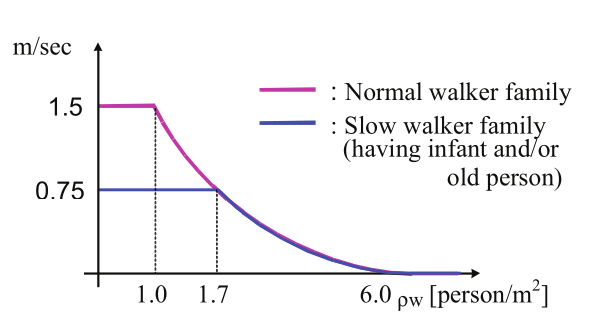
\includegraphics[width=\textwidth]{images/speed_GOTO.png}
        \caption{}
        \label{fig:goto-ped}
    \end{subfigure}
    \hfill
    \begin{subfigure}{0.32\textwidth}
        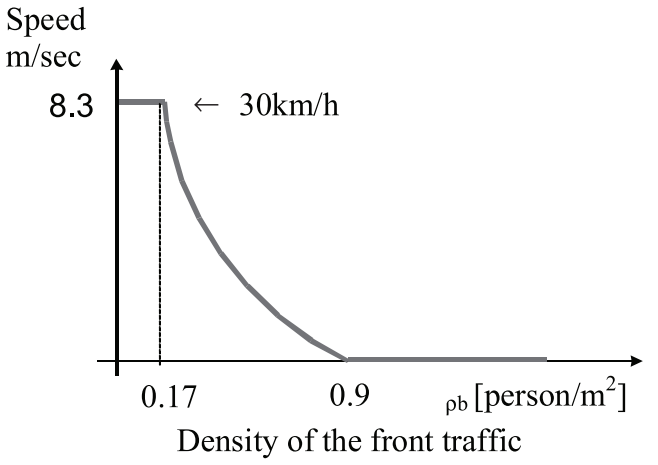
\includegraphics[width=\textwidth]{images/speed_GOTO_motocicli.png}
        \caption{}
        \label{fig:goto-moto}
    \end{subfigure}
    \hfill
    \begin{subfigure}{0.32\textwidth}
        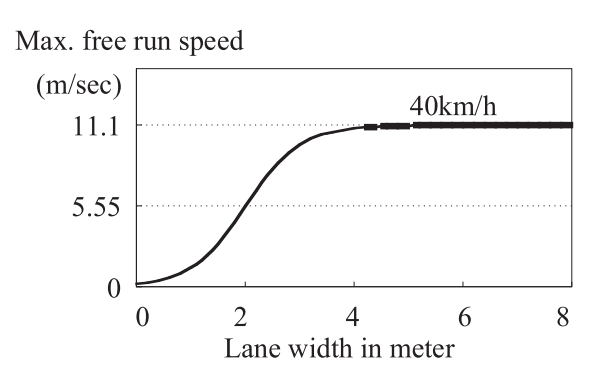
\includegraphics[width=\textwidth]{images/speed_GOTO_auto.png}
        \caption{}
        \label{fig:goto-auto}
    \end{subfigure}
    \caption{Relazione velocità-densità di \textcite{goto2012tsunami} per i pedoni (a), per i motocicli (b), e velocità massima per le auto in base alla larghezza della strada (c).}
    \label{fig:ankdasndk}
\end{figure}

I pedoni sono distinti in \textit{normal walkers}, con velocità massima di 1.5 m/s, e
\textit{slow walkers} (famiglie con disabili, anziani o bambini), con velocità massima di 0.75 m/s.
%
La velocità viene aggiornata al variare della densità con un massimo di $6 p/m^2$ (Fig. \ref{fig:goto-ped}).

Per i motocicli è stata considerata una velocità massima di 30km/h e una densità massima di 0.9 $p/m^2$ (Fig. \ref{fig:goto-moto}).

Per pedoni e motocicli la densità viene calcolata tramite la seguente formula:
$\rho = n /(L \times W)$, dove $n$ è il numero di agenti nell'area di fronte all'agente $L \times W$, $L$ è la lunghezza di ricerca 
e $W$ la larghezza della strada.

\begin{figure}[ht]
    \centering
    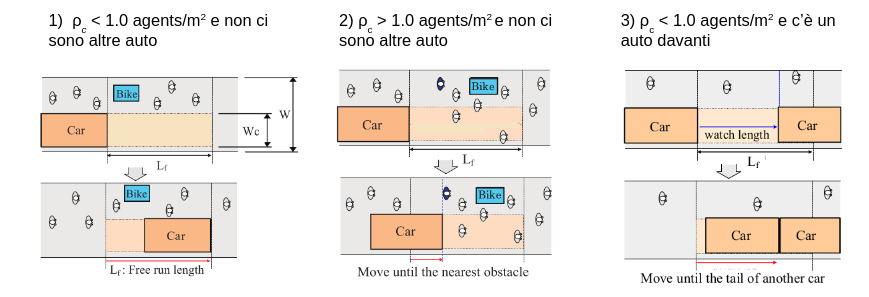
\includegraphics[width=\textwidth]{images/goto_car.png}
    \caption{Diversi casi che descrivono fino a dove l'auto si può muovere, in base alla densità e alla presenza di altre auto di fronte \parencite{goto2012tsunami}.}
    \label{fig:goto-car-model}
\end{figure}

Le auto in assenza di ostacoli si muovono per $L_{f} = V_{f} \times \Delta_{t} $, dove $L_{f}$ è la \textit{free run length},
$V_{f}$ la velocità massima e $\Delta_{t}$ il \textit{time step}.
La velocità massima cambia in base alla larghezza della strada con un limite di 40 km/h (Fig. \ref{fig:goto-auto}).

Per le auto la densità è definita da $\rho = n /((W - W_{c}) x L_{f})$, dove $W_{c}$ è la larghezza di un' auto.
La densità di un'auto viene considerata 10 volte quella di un pedone, mentre di una moto 2 volte quella di un pedone.

In base alla densità l'auto si muoverà fino al prossimo ostacolo, oppure fino alla prossima auto se presente (Fig. \ref{fig:goto-car-model}).

\subsection{Mostafizi, Wang et. al}
In questa sezione verrà descritto brevemente il modello di \textcite{wang2016agent} in quanto è stato scelto come modello di partenza per questo lavoro.
Inoltre verranno mostrate alcune modifiche effettuate in altri lavori degli stessi autori.

\subsubsection*{Wang et. al (2016)}

Nel lavoro di \textcite{wang2016agent} viene studiato come il tempo di preparazione, la scelta della modalità di evacuazione, la velocità dei pedoni e la 
presenza di rifugi per l'evacuazione verticale influenzi la quantità di vittime.

Al contrario del modello di \textcite{goto2012tsunami} viene considerato un numero molto limitato di agenti, ovvero 4502 individui. 
Inoltre i rifugi si assume che abbiano capacità illimitata e che non subiscano danni sismici. 

Come nel lavoro di \textcite{goto2012tsunami} il routing avviene tramite il percorso più breve e viene considerato lo stesso casualty model.

\pagebreak

Il modello gestisce due tipi di agenti: auto e pedoni. Le interazioni tra questi tipi di agenti sono limitate.
I pedoni hanno velocità costante definita secondo una distribuzione normale, e le auto interagiscono tra loro 
tramite il modello \textit{General Motors}. Quindi non è gestita nessuna interazione pedone-pedone e pedone-auto.


% Questo modello verrà descritto brevemente in quanto selezionato come modello di partenza per questo lavoro e nella sezione successiva.
% Questo modello consiste di un numero molto limitato di agenti rispetto al modello di \textcite{goto2012tsunami}, 4502 individui.
% Viene analizzato come l'aggiunta di rifugi verticali modalità
% Anche qui il routing avviene mediate l'utilizzo del percorso più breve ed lo stesso casualty model viene considerato, 
% mentre gli shelter si assume abbiano capacità illimitata.

% Al contrario di \textcite{goto2012tsunami} le interazioni tra i diversi tipi di agenti sono abbastanza limitate.
% I pedoni hanno velocità costante definita secondo una distribuzione normale, mentre le auto interagiscono tra di loro secondo il modello \textit{General Motors}.
% Infine non avendo dati sul quali fare validazione gli autori si sono limitati ad uno studio 
% dell'impatto sulla mortalità dato dai diversi parametri del modello tempi di preparazione, velocità dei pedoni e modalità di evacuazione.

\subsubsection*{Mostafizi, et. al. (2017)}
Il lavoro di \textcite{mostafizi2017agent} è basato sul precedente \parencite{wang2016agent} e si focalizza sul misurare la resilienza della rete stradale tramite l'analisi della mortalità.

Per i tempi di preparazione viene considarata una situazione ideale in cui gli agenti evacuano immediatamente dopo l'allarme. Inoltre per poter rappresentare
meglio il rischio per persone anziane o bambini, la profondità critica per il casualty model è stata ridotta a 0.5 m.

Ogni scenario è stato simulato molteplici volte per catturare la randomicità dei parametri. 
Per misurare il contributo di ogni link alla mortalità totale è stata considerata la mortalità media per ogni scenario al variare del numero di auto e pedoni.
I link critici sono stati identificati come quelli con una percentuale di mortalità superiore al 5\% sulla media di ogni combinazione di agenti.

\subsubsection*{Mostafizi, et. al. (2019)}
Il lavoro di \textcite{mostafizi2019agent} si basa sui due lavori precedenti e 
presenta un'analisi di sensitività di diversi fattori. 
In aggiunta ai precedenti lavori sono stati analizzati diversi parametri per 
il modello \textit{General Motors} e diversi limiti di velocità per le auto.


\subsection{Z. Wang e Jia (2021)}
In questo lavoro viene proposto un modello di evacuazione multimodale e una valutazione dei rischi modellando l'incertezza
nei danni sismici nelle strade e nei parametri del modello. Inoltre viene introdotta una velocità variabile per i pedoni e sono state 
gestite le interazioni tra auto e pedoni.

Sono state considerate diverse popolazioni al variare del numero di agenti: 5000 e 10,000,
che rappresentano la popolazione all'inizio dell'estate e 15,000 rappresenta il picco nella stagione estiva.

Gli agenti sono distinti in pedoni e auto ed evacuano verso il rifugio più vicino seguendo il percorso più breve.
Ogni auto contiene 4 persone ed è equivalente a 10 volte un pedone in spazio occupato.
Gli agenti per poter evacuare in auto dovranno prima raggiungere a piedi degli appositi parcheggi.

La velocità per i pedoni è distribuita secondo una normale $\mathcal{N}(\mu_p,\sigma_p)$ troncata tra 0.75 m/s e 3.83 m/s e
con $\mu_p \sim \mathcal{U}(1.4, 2)$ e $\sigma_p \sim \mathcal{U}(0.1, 0.6)$.
Inoltre viene aggiornata in base alla densità di fronte all'agente con una \textit{search length} di 4m secondo l'andamento mostrato in figura \ref{fig:wang2021}.

\begin{figure}[ht]
    \centering
    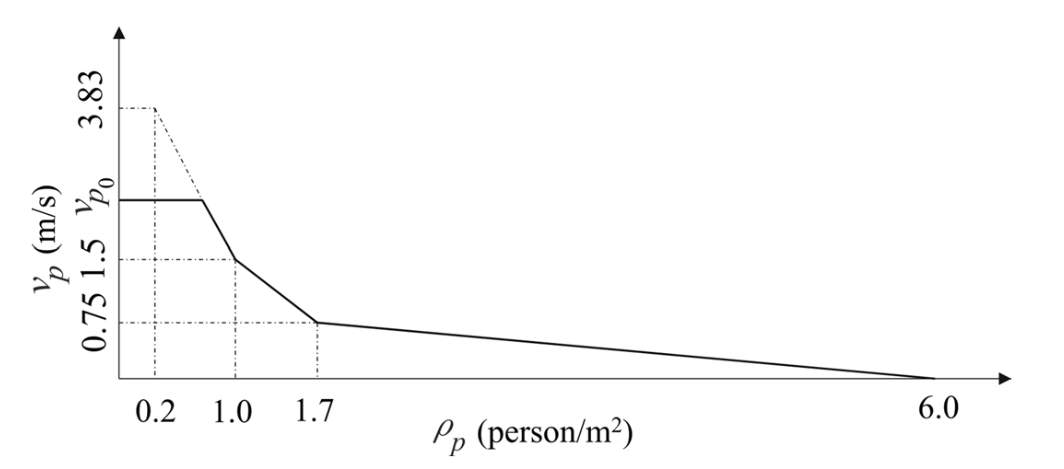
\includegraphics[width=0.7\textwidth]{images/speed_WANG.png}
    \caption{Relazione velocità-densità di \textcite{wang2021novel} basata su un'approssimazione del modello di \textcite{goto2012tsunami}.}
    \label{fig:wang2021}
\end{figure}

Per le auto è stato utilizzato il modello di \textcite{greenshields1935study} che aggiorna la velocità in base alla densità di fronte lungo la \textit{free run length},
con una massima velocità di 40 km/h e una densità massima di 160 veh/km per i link senza restrizioni sul traffico date dai danni sismici.

Per la gestione delle interazioni tra auto e pedoni vengono definite tre fasi di traffico in base al rapporto
tra il volume dei pedoni e delle auto: \textit{vehicle-dominated}, \textit{balanced} e \textit{pedestrian-dominated}.
Al variare della fase cambia la larghezza della strada occupabile sia per pedoni che per le auto.

Per gestire i danni sismici viene assegnato un livello di distruzione ad ogni link e sulla base di questo viene 
ridotta la capacità massima riducendo la densità massima.

Per i tempi di partenza viene utilizzata la distribuzione di Rayleigh dove i parametri
invece di essere fissati seguono delle apposite distribuzioni uniformi.

Rispetto ad altri lavori che utilizzano un livello di profondità fissa per determinare la morte degli agenti, in questo lavoro
viene considerato che la profondità sia distribuita uniformemente in [0.5, 3]. 

\section{Descrizione del Modello}
\label{sec:modello}
In questa sezione verranno descritti i diversi agenti e l'ambiente.
I parametri usati per questo lavoro saranno specificati nella sezione \ref{sec:simulazione}.

Il modello considerato \parencite{mostafizi2016agent} è un sistema multi-agente che prevede l'evacuazione della città di Seaside, Oregon in caso di tsunami di auto e pedoni.
%
L'evacuazione inizia subito dopo il terremoto e non vengono considerati eventuali danni causati dal terremoto.

\pagebreak

Il modello utilizza dati GIS per la distribuzione della popolazione, la rete stradale e i rifugi.
%
Per la distribuzione della popolazione è stato considerato uno scenario a mezzogiorno di un fine settimana di estate,
che presenta una maggiore concentrazione di residenti sulla spiaggia e nel centro della città.
La popolazione sulla costa (40\%) e nel centro (30\%) è distribuita normalmente,
mentre quella nella zona residenziale (30\%) è distribuita uniformemente (Fig. \ref{fig:population}).

\begin{figure}[ht]
  \centering
  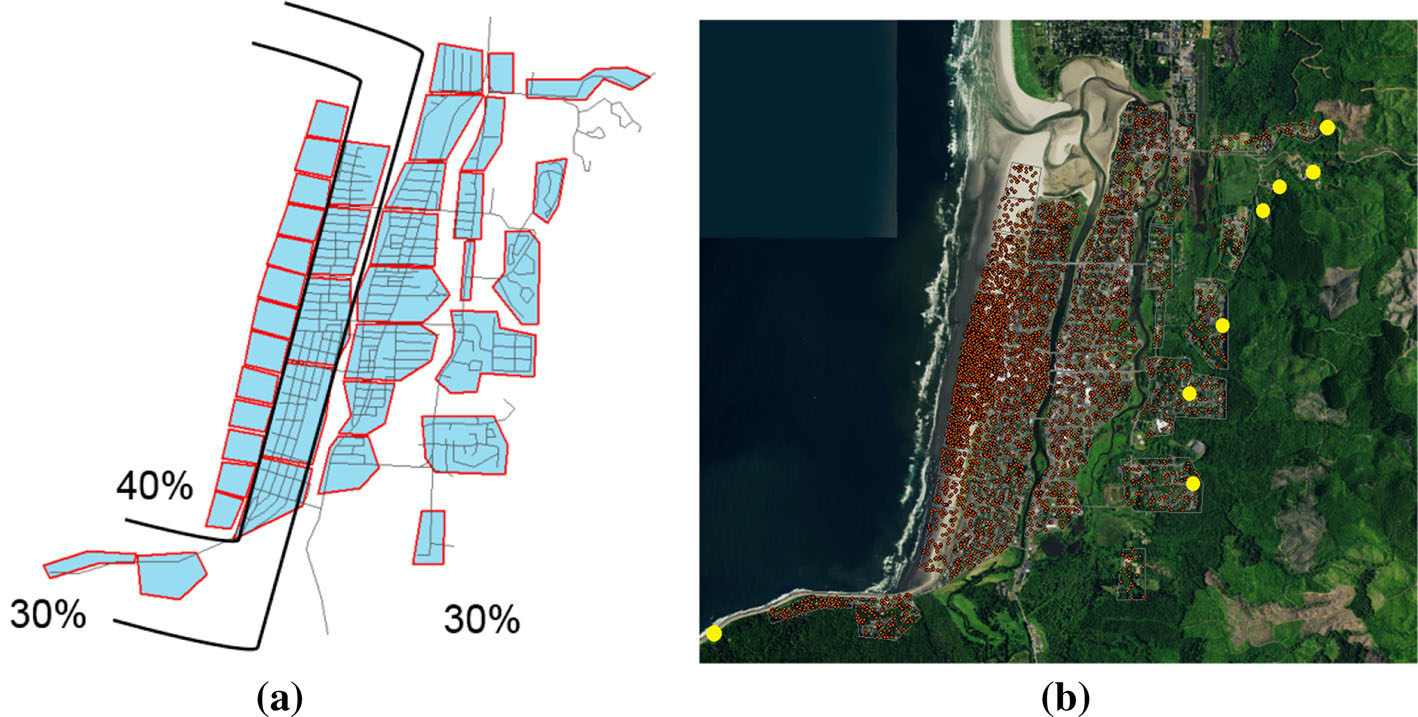
\includegraphics[width=0.82\textwidth]{images/population}
  \caption{Distribuzione della popolazione nello scenario considerato.
    (a) Aree in cui è distribuita la popolazione divise nelle tre macro aree: costa, centro, zona residenziale.
    (b) Immagine satellitare con la distribuzione della popolazione.}
  \label{fig:population}
\end{figure}

\subsection{Ambiente}
L'ambiente è composto dalla rete stradale della città con i relativi rifugi e dallo tsunami.

La rete stradale è rappresentata da un grafo, i cui nodi corrispondono alle intersezioni e gli archi alle strade.
Tutte le strade sono considerate a senso unico, con una sola corsia e con una velocità limite di 55 km/h e hanno una lunghezza fissata.
8 delle intersezioni sono marcate come rifugi con capacità illimitata.

Lo tsunami è rappresentato da una griglia discreta, dove ogni cella contiene i valori temporali di altezza delle onde.
I dati usati in questo progetto sono quelli calcolati dal modello di inondazione ComMIT/MOST \parencite{titov1997implementation} per la zona di subduzione della Cascadia.

\pagebreak

\subsection{Agenti}
La simulazione prevede diversi tipi di agenti: residenti, pedoni e auto.

\subsubsection{Residenti}
All'inizio dell'evacuazione i residenti si trovano all'esterno degli edifici e delle auto
e scelgono come evacuare autonomamente.
Un residente sceglie con una certa probabilità la modalità per evacuare: a piedi o in auto e verso un rifugio verticale oppure orizzontale.
Una volta che ogni agente decide in che modo evacuare non cambierà scelta per tutta la simulazione.

Prima di iniziare l'evacuazione i residenti impiegano del tempo per prepararsi
che include l'eventuale raggiungimento del veicolo.
%
Questo tempo, chiamato \textit{milling time}, è modellato tramite
la distribuzione di Rayleigh (Eq. \ref{eq:rayleigh}), con un tempo minimo di preparazione ($\tau$) e un parametro di scala ($\sigma$).

\begin{equation}
  P(t) = 
  \begin{cases}
    0 &0 < t < \tau\\
    1 - e^{-{(t - \tau)^2}/(2\sigma^2)} &t \geq \tau
  \end{cases}
  \label{eq:rayleigh}
\end{equation}

Scaduto il tempo di preparazione l'agente si muove verso l'intersezione più vicina e
in base alla modalità scelta viene considerato un agente di tipo pedone o auto.
L'agente quindi inizia a seguire il percorso più breve per il rifugio più vicino raggiungibile, trovato tramite l'algoritmo A* 
che prende in considerazione esclusivamente la lunghezza delle strade.

\vspace*{4mm}

\noindent
Gli agenti durante l'evacuazione possono:
\begin{itemize}
  \item Continuare sulla strada attuale.
  \item Cambiare strada seguendo il percorso più breve.
  \item Morire se l'altezza delle onde supera $H_c$.
  \item Evacuare se hanno raggiunto un rifugio.
\end{itemize}

\subsubsection{Pedoni}
La velocità di camminata viene stabilita tramite una distribuzione normale
con media $\mu_p$ e deviazione standard $\sigma_p$, in questo modo vengono considerati diversi tipi di pedoni dai più veloci ai più lenti.
La velocità di ogni pedone rimane costante durante tutta l'evacuazione.

\begin{figure}[ht]
  \centering
  \includegraphics[width=0.8\textwidth]{images/modello_base_velocità_pedoni.png}
  \label{fig:modello-base-velocità-pedoni-img}
  \caption{Differenti distribuzioni di velocità al variare di $\mu_p$ e $\sigma_p$.}
\end{figure}

\subsubsection{Auto}
È stato considerato il caso peggiore in cui ogni auto contiene una sola persona.
Le auto possono raggiungere la velocità massima imposta dalla strada, ovvero 55 km/h.

Il comportamento delle auto è modellato tramite il modello \textit{General Motors} il quale fa parte dei modelli
di tipo \textit{car-following}. Questi modelli descrivono come un veicolo ne segue un altro
e cambi il proprio comportamenteo reagendo a quest'ultimo.

\begin{figure}[ht]
  \centering
  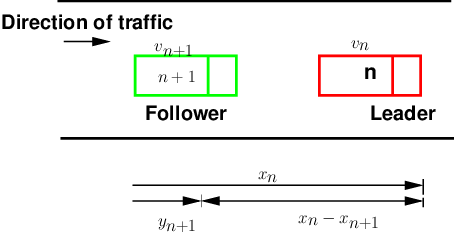
\includegraphics[width=0.6\textwidth]{images/GM.png}
  \label{fig:general-motors-img}
  \caption{Schema generale dei modelli \textit{car-following}, dove $n+1$ è il veicolo corrente e $n$ quello di fronte, 
  $v_{n+1}, v_{n}$ sono le rispettive velocità, mentre $x_{n+1}, x_{n}$ sono le rispettive posizioni e $x_{n} - x_{n + 1}$ è la distanza tra i due veicoli.}
\end{figure}

Secondo il modello General Motors ogni auto risponde alle condizioni del traffico circostante esclusivamente accelerando o decelerando. 
L'accelerazione dipende dalla velocità del veicolo corrente, dalla sua posizione e dalla sua velocità rispetto al veicolo di fronte.

Più veloce è il veicolo di fronte maggiore sarà la distanza tra i due veicoli,
e inoltre deve essere mantenuta una certa distanza di sicurezza dall'auto di fronte.

\begin{equation}
  a_{n+1}^{t} = [ \frac{\alpha_{l, m} * (v_{n + 1}^{t})^{m} }{ (x_{n}^{t} - x_{n + 1}^{t})^{l}}][v_{n}^{t} - v_{n + 1}^{t}]
  \label{eq:general-motors-eq}
\end{equation}

L'equazione \ref{eq:general-motors-eq} mostra il modello \textit{General Motors},
dove $l$ è un esponente di distanza con il veicolo di fronte che può assumere valori da +4 a -1,
$m$ è un esponente di velocità con valori tra -2 a +2, $\alpha$ è un coefficiente di sensitività.

\section{Estensione del Modello}
In questa sezione verrano descritte le modifiche e le aggiunte effettuate al modello base,
% TODO: riscrivere
ma prima verrano evidenziate le limitazioni e le mancanze del modello anche rispetto allo stato dell'arte.

Molte assunzioni sono poco realistiche come la velocità costante dei pedoni, tutte le strade a senso unico e l'assenza di interazioni nelle
intersezioni.
%
Inoltre viene assunto che tutti gli agenti conoscano il percorso più breve per il rifugio.
%
Un'altra limitazione riguarda le interazioni tra i vari tipi di agenti.
Questo modello considera esclusivamente le interazioni auto-auto
tramite il modello General Motors, ma non prevede nessuna interazione pedone-pedone o pedone-auto.

% TODO: riscrivere
Come è stato appena descritto le interazioni tra gli agenti
hanno un ampio margine per essere ?rappresentate?, in particolare ci si concentrerà sulle interazioni nelle intersezioni
introducendo meccanismi di coordinazione tra i vari tipi di agente. Inoltre la velocità dei pedoni verrà modificata in base alla congestione
in modo da poter rappresentare uno scenario più realistico.

\subsection{Rete Stradale}
Prima di descrivere le varie aggiunte in questa sezione verrannò elencate le varie modifiche che sono state effettuate alla rete stradale.

Tutte le strade della rete sono state considerate come strade locali secondo il \textcite{seaside2010tsp},
ovvero strade a doppio senso e a una corsia con una larghezza variabile da 7.3 m a 9 m e opzionalmente
un marciapiedie per ogni lato della strada con una larghezza fissa di 1.5 m.
%
È stato assunto che tutte le strade abbiano marciapiedi su entrambi i lati e che la larghezza sia fissata al valore minimo.

% TODO: espandere
Sono stati associati gli stop alle strade collegate ad un intersezioni.

\subsection{Speed Variability dei Pedoni}
Riassunto stato dell'arte per la speed variability e survey di modelli macroscopici sui diagrammi fondamentali.

È stata introdotta una variabilità nella velocità di camminata per i pedoni utilizzando il modello di Weiddman con una \textit{free flow speed} di 1.34 m/s
e una \textit{jam density} di 5.4 p/m².
Il calcolo della densità è stato effettuato considerando un'area di ricerca di 4 m x 1.5 m di fronte al pedone,
come in \textcite{goto2012tsunami, wang2021novel}.

I pedoni nel caso in cui sono presenti anche auto, procedono esclusivamente sui marciapiedi, altrimenti occupano tutta la strada.

Spiegare modello di weidmann.

\newpage

\subsection{Gestione degli Intersezioni}
Per la gestione delle intersezioni sono stati considerati esclusivamente gli incroci a 4 strade e trattati come intersezioni di tipo AWSC (All Way Stop Controlled) o TWSC (Two Way Stop controlled).

% TODO: riscrivere, un po' confuso
Tramite l'utilizzo di OpenStreetMap e GoogleMaps, sono state estratte manualmente le informazioni circa la posizione e nel case dei TWSC la direzione
di precedenza di tali tipi di incroci per la citta di Seaside, ottenendo la seguente (Fig. \ref{fig:intersections}).

\begin{figure}
    \centering
    \begin{subfigure}{0.475\textwidth}
        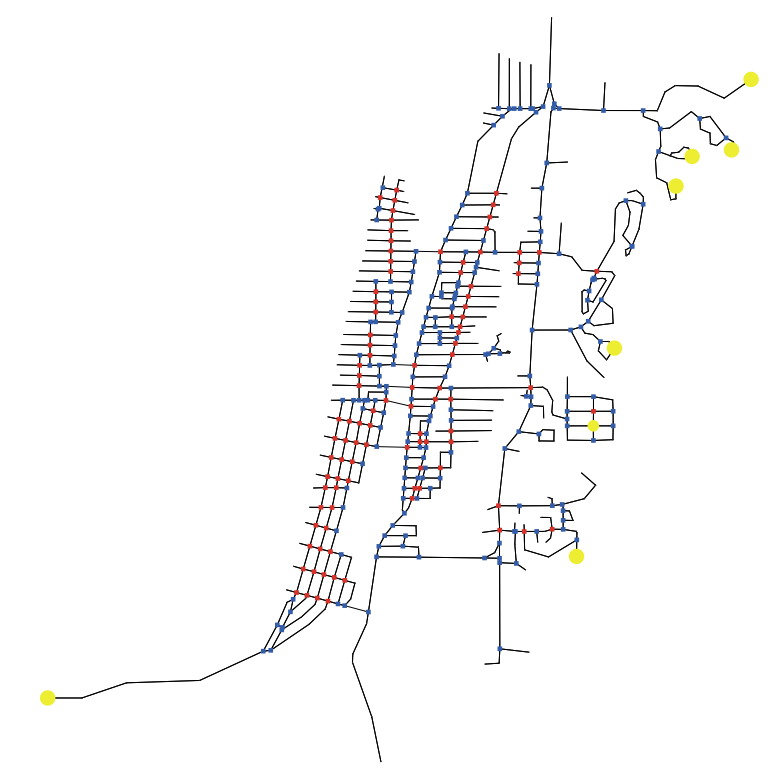
\includegraphics[width=\textwidth]{images/intersections}
        \caption{intersezioni classificate per numero di strade: verde a 4 strade (98 nodi) e grigio a 3 strade (206 nodi).}
        \label{fig:intersections}
    \end{subfigure}
    \hfill
    \begin{subfigure}{0.475\textwidth}
        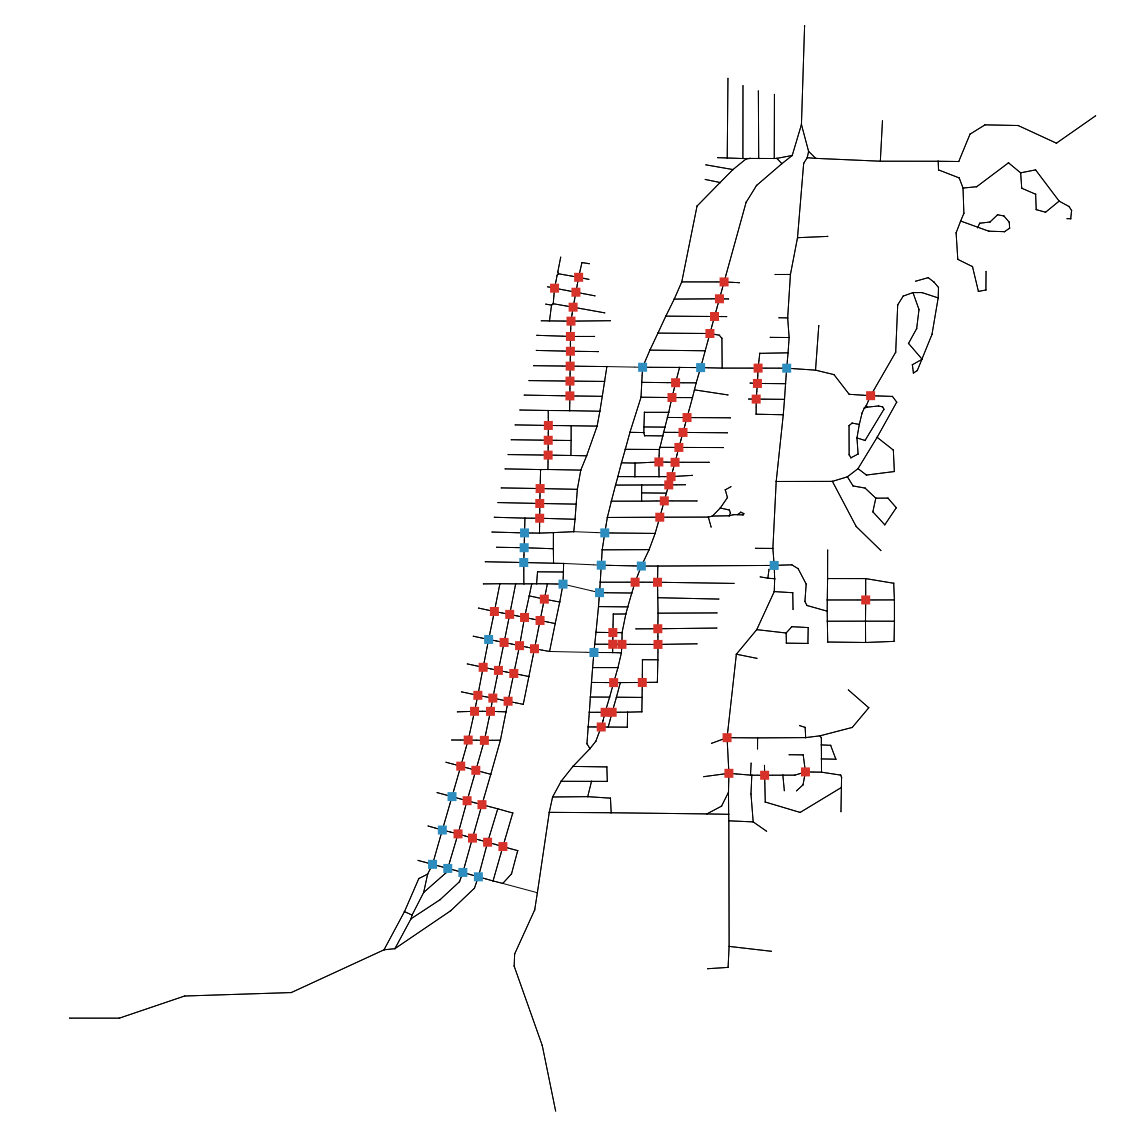
\includegraphics[width=\textwidth]{images/int_type}
        \caption{intersezioni a 4 strade classificate in base al tipo: AWSC in blu (20 nodi) e TWSC in rosso (78 nodi).}
        \label{fig:intersections_types}
    \end{subfigure}
    \caption{Tipi di intersezioni.}
\end{figure}

Inoltre nelle intersezioni è stata introdotta una zona di attraversamento per la gestione delle interazioni tra auto e pedoni.
È stato assunto che gli incroci abbiano lunghezza e larghezza pari alla larghezza della strada (10.3 m).
Dal momento che la rappresentazione della strada è network-based è stato deciso che
la zona iniza prima dell'incrocio e finisce dopo dell'incrocio a una distanza pari alla metà della larghezza (5.15 m) (Fig. \ref{fig:crossing-area}).

\begin{figure}[ht]
    \centering
    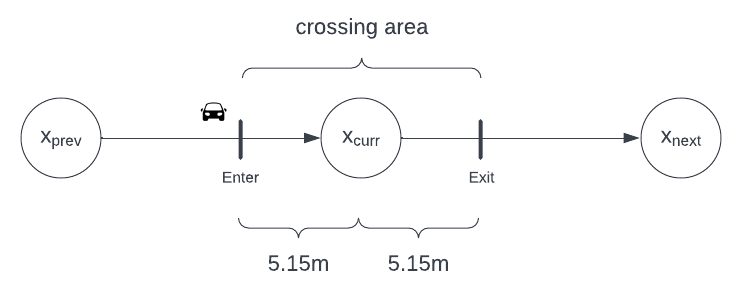
\includegraphics[width=0.5\textwidth]{images/crossing_area}
    \caption{Zona di attraversamento di un'intersezione.}
    \label{fig:crossing-area}
\end{figure}

\newpage
Per rappresentare l'attraversamento dei pedoni e delle auto sono state aggiunte le seguenti informazioni ad ogni intersezione $i$ a 4 strade:
\begin{itemize}
    \item $C_{i, j}$ = numero di pedoni che stanno usando l'attraversamento pedonale che si trova sulla strada che va dall'incrocio $i$ all'incrocio $j$.
    \item $\textit{Arrival}_i$ = coda delle auto nella zona di attraversamento ordinate per tempo di arrivo.
    \item $\textit{Crossing}_i$ = insieme delle auto che possono passare contemporaneamente.
    \item $\textit{Stops}_i$ = insieme delle intersezioni $j$ collegate a $i$ in cui è presente uno stop nella strada $(i, j)$.
\end{itemize}

% Inoltre per i TWSC nelle intersezioni la presenza degli stop viene segnata, mediante una lista con il numero dell'intersezioni interessate.

Per stabilire la posizione all'interno della rete stradale, le precedenze e la direzione della prossima intersezione per ogni agente $x$
vengono definite:
\begin{itemize}
    \item $x_{prev}$ l'intersezione precendente
    \item $x_{curr}$ l'intersezione corrente
    \item $x_{next}$ la prossima intersezione
    \item $x_{side} \in \{ \textit{left}, \textit{right} \}$  il lato di marciapiede (solo pedoni)
    \item $x_{xdir} \in \{\textit{left}, \textit{straight}, \textit{right}\}$ la direzione verso $x_{next}$
\end{itemize}

\newpage
\subsubsection{Pedoni}
% Dato un pedone $x$ si definiscono $x_{prev}$ l'intersezione precendente, $x_{curr}$ l'intersezione corrente e $x_{next}$ la prossima intersezione.

Data la tripla ($x_{prev}$, $x_{curr}$, $x_{next}$) viene associata ad ogni intersezione collegata a $x_{curr}$ la direzione per raggiungerla seguendo il senso orario a partire da $x_{prev}$,
per cui $I_d$ indica l'intersezione nella direzione $d \in \{\textit{origin}, \textit{left}, \textit{straight}, \textit{right}\}$.
%
La direzione associata all'intersezione $x_{next}$ è quella dove è diretto il pedone e viene identificata da $x_{dir}$.

Quando un pedone $x$ entra nella zona di attraversamento di $x_{curr}$ dall'intersezione $x_{prev}$ e si trova sul marciapiede $x_{side}$
ha tre direzioni in cui poter andare: \textit{left}, \textit{straight}, \textit{right} (Fig. \ref{fig:pedestria-crossing}):
\begin{itemize}
    \item Se $x_{dir} = \textit{straight}$ e $x_{side} = \textit{side}$ viene incrementato $C_{x_{curr}, I_{\textit{side}}}$ di 1.
    \item Se $x_{dir} = \textit{side}$ e $x_{side} \neq \textit{side}$ viene incrementato $C_{x_{curr}, I_{\textit{origin}}}$ di 1.
    \item Se  $x_{dir} = \textit{side}$ e $x_{side} = \textit{side}$ non viene alterato nessun contatore.
\end{itemize}

Quando il pedone finisce di attraversare il contatore corrispondente viene decrementato di 1.


\begin{figure}[ht]
    \centering
    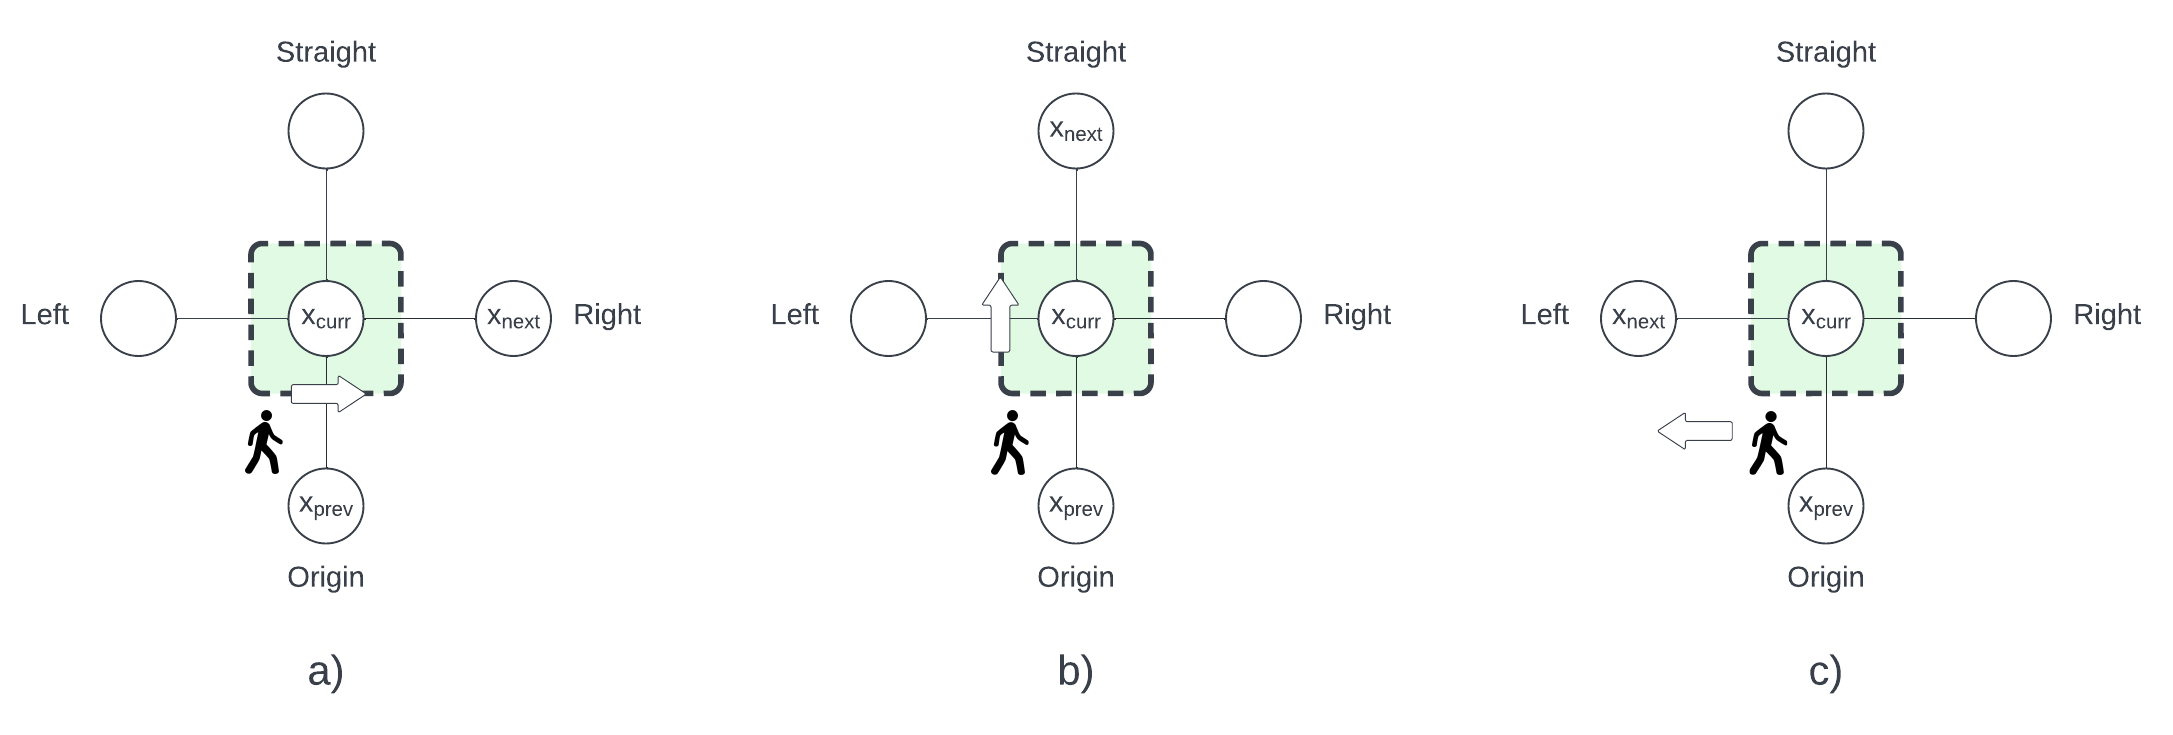
\includegraphics[width=\textwidth]{images/pedestrian_crossing}
    \caption{
        Esempio dei tre casi di attraversamento dal punto di vista del pedone che si trova sul marciapiede sinistro.
        a) il pedone si trova sul lato sinistro e attraversa sul link collegato a origin.
        b) il pedone attraverso sul lato sinistro dell'incrocio, quindi sul link collegato a left.
        c) il pedone segue il marciapiede sulla sinistra senza attraversare.
    }
    \label{fig:pedestria-crossing}
\end{figure}


\subsubsection{Auto}
Quando un auto $x$ raggiunge la zona di attraversamento dell'intersezione $i$ viene aggiunta alla coda $\textit{Arrival}_i$ che
determina l'ordine di arrivo delle auto. In base al tipo di intersezione viene schedulata e una volta avuto il via libera
viene aggiunta a $\textit{Crossing}_i$ e rimossa una volta lasciato l'incrocio.

Le auto quando raggiungono la zona di attraversamento vengono aggiunte alla coda $\textit{Arrival}_i$ e schedulate
in base al tipo d'intersezione (Sec. \ref{subsubsec:precedenze}), una volta avuto il via libera le auto sono aggiunte a $\textit{Crossing}_i$
e rimosse una volta lasciato l'incrocio.
%
Se ci sono pedoni che stanno attraversando le strade $(x_{curr}, x_{next})$ e $(x_{prev}, x_{curr})$ l'auto dovrà attendere,
quindi potrà passare se e solo se $C_{x_{curr},x_{prev}}$ = 0 e $C_{x_{curr},x_{next}}$ = 0 (Fig. \ref{fig:auto-ped-crossing}).

\begin{figure}[ht]
    \centering
    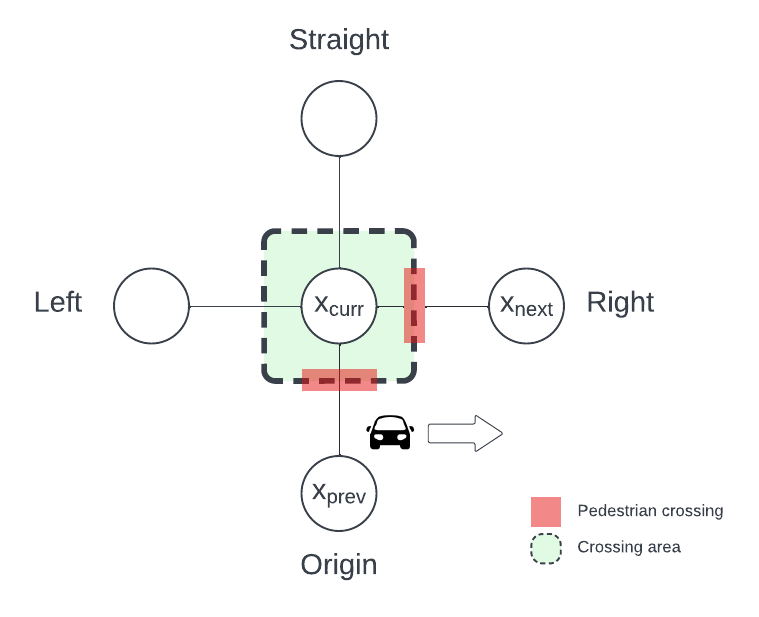
\includegraphics[width=0.45\textwidth]{images/crossing_auto_ped_crossing}
    \caption{Esempio degli attraversamenti pedonali (in rosso) che vanno controllati
        per poter passare data la tripla ($x_{prev}$, $x_{curr}$, $x_{next}$) di un auto $x$.}
    \label{fig:auto-ped-crossing}
\end{figure}

\subsubsection{AWSC}
\label{subsubsec:precedenze}
Nelle intersezioni di tipo AWSC la prima auto che arriva ha la precedenza sulle altre auto e deve aspettare eventuali pedoni come spiegato in precedenza.
Inoltre lo scenario in cui 4 auto arrivano contemporaneamente non è stato considerato poiché poco probabile.

La risoluzione delle precedenze avviene tra le auto che arrivano a un'intersezione allo stesso tempo.
L'auto che ha la destra libera viene considerata provenire da \textit{origin} e dal suo punto di riferimento
vengono identificate le direzioni di provenienza delle altre auto.

Basandosi sulle direzioni di provenienza delle auto e sulle rispettive destinazioni viene verificato
in senso orario (\textit{origin} $\rightarrow$ \textit{left} $\rightarrow$ \textit{straight})
quali auto possono passare contemporaneamente o meno (Tab. \ref{tab:origin-left}, Tab. \ref{tab:origin-straight}, Tab. \ref{tab:origin-left-straight}).


\begin{table}[ht]
    \centering
    \begin{tabular}{|c|c|c|}
        \hline
        \textbf{Car1: Origin} & \textbf{Car2: Left} \\ \hline
        Left                  & Left                \\ \hline
        Right                 & Right               \\ \hline
        Right                 & Straight            \\ \hline
        Straight              & Right               \\ \hline
    \end{tabular}
    \caption{Tutte le possibili combinazioni di destinazione delle due auto che permettono
        di passare contemporaneamente nel caso in cui arrivano rispettivamente da \textit{origin} e \textit{left}.}
    \label{tab:origin-left}
\end{table}

\begin{table}[ht]
    \centering
    \begin{tabular}{|c|c|c|}
        \hline
        \textbf{Car1: Origin} & \textbf{Car2: Straight} \\ \hline
        Left                  & Right                   \\ \hline
        Right                 & Left                    \\ \hline
        Right                 & Right                   \\ \hline
        Straight              & Right                   \\ \hline
    \end{tabular}
    \caption{Tutte le possibili combinazioni di destinazione delle due auto che permettono
        di passare contemporaneamente nel caso in cui arrivano rispettivamente da \textit{origin} e \textit{straight}.}
    \label{tab:origin-straight}
\end{table}

\begin{table}[ht]
    \centering
    \begin{tabular}{|c|c|c|}
        \hline
        \textbf{Car1: Origin} & \textbf{Car2: Left} & \textbf{Car3: Straight} \\ \hline
        Right                 & Left                & Right                   \\ \hline
        Left                  & Right               & Left                    \\ \hline
        Right                 & Right               & Right                   \\ \hline
        Straight              & Right               & Right                   \\ \hline
    \end{tabular}
    \caption{Tutte le possibili combinazioni di destinazione delle tre auto che permettono
        di passare contemporaneamente nel caso in cui arrivano rispettivamente da \textit{origin}, \textit{left} e \textit{straight}.}
    \label{tab:origin-left-straight}
\end{table}

\subsubsection{TWSC}
Nel caso in cui l'intersezione è di tipo TWSC vengono identificate due vie: quella principale che ha la precedenza e quella
secondaria in cui sono presenti gli stop.

A differenza dell'intersezioni AWSC, l'ordine di precedenza non importa poiché possono passare al più due auto alla volta
che si trovano l'una di fronte all'altra.
Quindi viene scelta casualmente come riferimento una delle due auto che viene considerata provenire da \textit{origin}, mentre
l'altra da \textit{straight}.
%
Una volta che la via principale è libera viene gestita nello stesso modo quella secondaria.

Per verificare se le due auto possono passare contemporaneamente si procede come già visto per il caso origin-straight (Tab. \ref{tab:origin-left-straight}).

\section{Simulazione}
\label{sec:simulazione}
Per la simulazione alcuni parametri sono stati fissati secondo il modello \parencite{mostafizi2017agent}, mentre altri parametri sono estratti randomicamente 
o sono stati cambiati manualmente per i diversi esperimenti.

\subsection{Parametri Fissati}
\label{ssec:parametri-fissi}

Parametri per il modello \textit{General Motors}:
\begin{itemize}
    \item \textbf{max speed}: 55 km/h. Velocità massima.
    \item \textbf{safe distance}: 1.8 m. Distanza minima tra le auto.
    \item \textbf{acceleration}: 1.5 m/s². Accelerazione nel caso in cui non è presente un'auto davanti.
    \item \textbf{l}: 2. Esponente di distanza.
    \item \textbf{m}: 0. Esponente di velocità.
    \item \textbf{alpha}: 0.36 km²/h. Coefficiente di sensitività. 
\end{itemize}

\noindent
Parametri per il \textit{casualty model}:
\begin{itemize}
  \item \textbf{Hc}: 0.5 m. Profondità critica alla quale l'agente viene considerato una vittima.
\end{itemize}

\noindent
Parametri per il tempo di preparazione:
\begin{itemize}
  \item \textbf{Rtau}: 1 min. Tempo minimo per prepararsi prima di evacuare.
  \item \textbf{Rsig}: 0.5. Fattore di scala per la distribuzione di Rayleigh.
\end{itemize}

\noindent
Parametri per il comportamento dei pedoni:
\begin{itemize}
  \item \textbf{search\_length}: 4 m. Lunghezza della strada davanti al pedone per calcolare la densità.
  \item \textbf{jam\_density}: 6 ped/m². Densità massima.
\end{itemize}

\noindent
Parametri per le dimensioni delle strade:
\begin{itemize}
  \item \textbf{side\_width}: 1.5 m. Larghezza di un marciapiede.
  \item \textbf{lane\_width}: 3.6 m. Larghezza di una corsia.
\end{itemize}

\subsection{Parametri Variabili}

Parametri per la percentuale di auto e pedoni:
\begin{itemize}
  \item \textbf{R1\_Evac\_Foot}: Probabilità di un residente di evacuare a piedi.
  \item \textbf{R2\_Evac\_Car}: Probabilità di un residente di evacuare in auto.
\end{itemize}

\noindent
Sono state provate le seguenti combinazioni di auto e pedoni:
\begin{itemize}
  \item \textbf{R1\_Evac\_Foot}: 0\%, \textbf{R2\_Evac\_Car}: 100\%
  \item \textbf{R1\_Evac\_Foot}: 25\%, \textbf{R2\_Evac\_Car}: 75\%
  \item \textbf{R1\_Evac\_Foot}: 50\%, \textbf{R2\_Evac\_Car}: 50\%
  \item \textbf{R1\_Evac\_Foot}: 75\%, \textbf{R2\_Evac\_Car}: 25\%
  \item \textbf{R1\_Evac\_Foot}: 100\%, \textbf{R2\_Evac\_Car}: 0\%
\end{itemize}

\noindent
Parametri per il comportamento dei pedoni:
\begin{itemize}
  \item \textbf{$\mu_p$}: 1.22 m/s. Velocità media.
  \item \textbf{$\sigma_p$}: 0.2. Deviazione standard della velocità.
  \item \textbf{side}: lato del marciapiede all'inizio della simulazione (0 sinistro e 1 destro), assegnato in modo equiprobabile. 
  Durante la simulazione può variare. 
\end{itemize}

\noindent
Per via della randomicità dei parametri i risultati degli esperimenti sono stati mediati su 30 simulazioni.

\section{Analisi}
\label{sec:analisi}
In questa sezione verrà effettuata un'analisi sui risultati mediati su 30 simulazioni, 
comparando il modello base con il modello esteso e infine con un modello allo stato dell'arte.

\subsection{Modello Base}
Nelle figure \ref{fig:analisi-base-evacuated} e \ref{fig:analisi-base-casualties} vengono mostrate le percentuali di evacuati 
e di morti nel tempo al variare del numero di auto e pedoni.
%
Come si può notare dalla figura \ref{fig:analisi-base-evacuated}, il numero di pedoni non influenza la percentuale di pedoni evacuati nel tempo.
%
Per quanto riguarda le auto, più è alto il numero di auto più tempo è richiesto per evacuare e inoltre più bassa è la percentuale di auto evacuate alla fine della simulazione.
%
Osservando la percentuale di evacuati totali si può notare che un numero minore di auto permette di evacuare il numero maggiore di agenti.
I casi con probabilità di pedoni del 75\% e 100\% si ottiene la stessa percentuale massima di agenti evacuati,
tuttavia il caso con probabilità 75\% ha un andamento più veloce per la presenza delle auto.

\begin{figure}[ht]
    \centering
    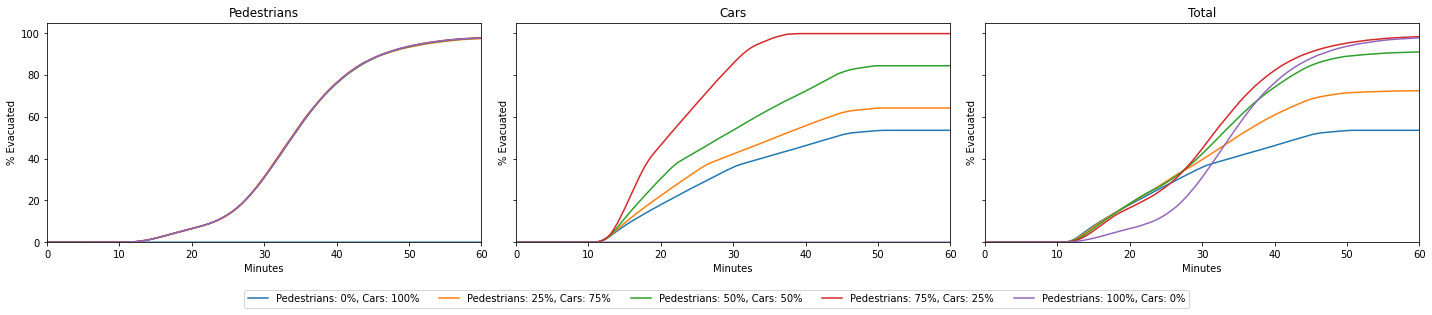
\includegraphics[width=\textwidth]{images/analisi/base-evacuated.png}
    \caption{Percentuale degli evacuati nel tempo al variare del numero di agenti con il modello base.}
    \label{fig:analisi-base-evacuated}
\end{figure}

% TODO: riscrivere
Per quanto riguarda le percentuali di mortalità (Fig. \ref{fig:analisi-base-casualties}), possono essere fatte analisi simili a quelle fatte in precendenza
per il numero di evacuati.
Per i pedoni in tutti i casi la percentuale di vittime rimane sotto al 2\%, mentre osservando le auto e le vittime totali
risulta una mortalità maggiore all'aumentare del numero di auto fino a un massimo di circa 50\%.
I casi con meno vittime sono con una probabilità di auto del 25\% e il caso solo pedoni che hanno risultati molto simili.

\begin{figure}[ht]
    \centering
    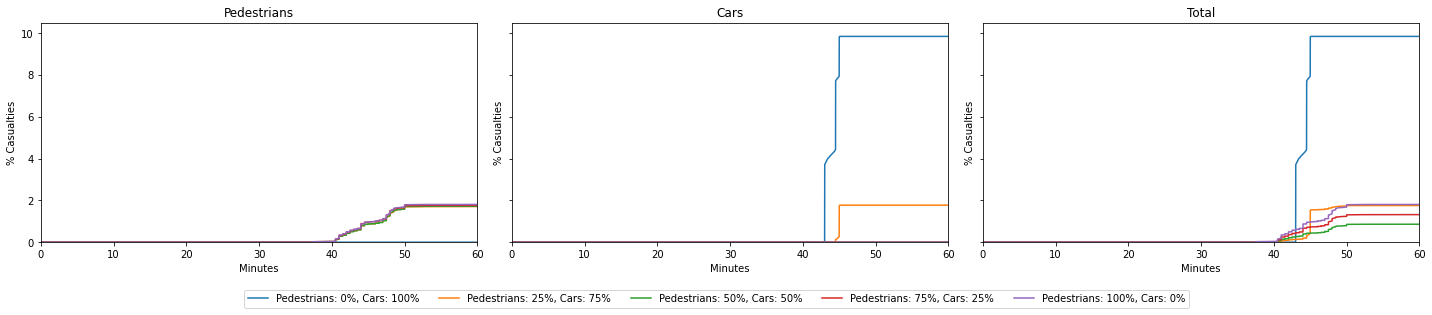
\includegraphics[width=\textwidth]{images/analisi/base-casualties.png}
    \caption{
        Percentuale delle vittime nel tempo al variare del numero di agenti con il modello base.
        %
    }
    \label{fig:analisi-base-casualties}
\end{figure}

Nella figura \ref{fig:analisi-base-evtimes} vengono riportate le percentuali di agenti evacuati nel tempo e il tempo in cui evacuano in media.
%
Nel caso con solo pedoni si ha un enorme picco al tempo medio di X minuti e all'aumentare del numero di auto 
il tempo medio di evacuzione si abbassa fino a X minuti nel caso con solo auto.

Nel caso con probabilità di auto del 25\% sembra formarsi un secondo picco più basso nei primi minuti probabilmente dovuto alle auto, mentre il secondo ai pedoni.
Questi picchi tendono ad appiattirsi con l'aumentare del numero di auto.

Inoltre si può notare come con un numero maggiore di auto considerate minore è la percentuale di agenti che evacuano negli ultimi minuti.
Questo poichè, come già evidenziato nella figura \ref{fig:analisi-base-evacuated}, le auto evacuano più velocemente dei pedoni.

\begin{figure}
    \centering
    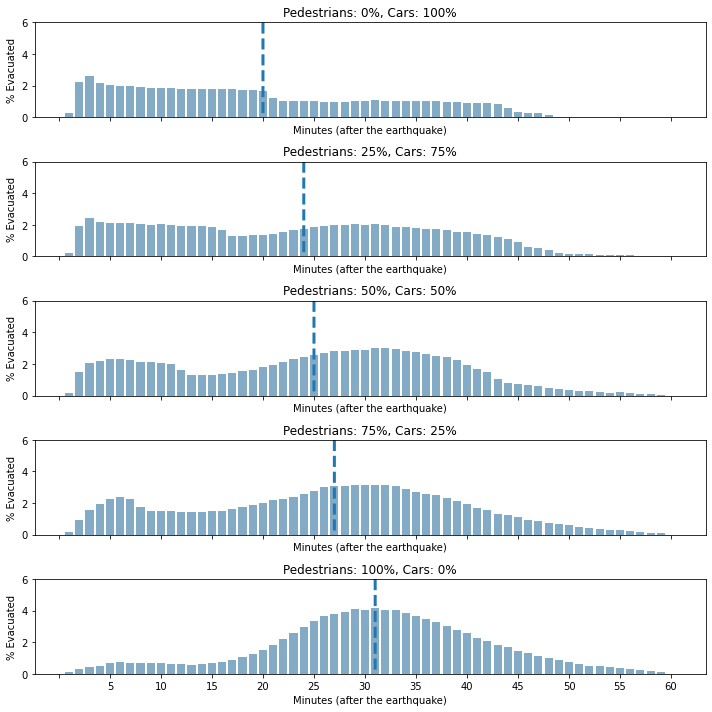
\includegraphics[width=\textwidth]{images/analisi/base-evtimes.png}
    \caption{
        Distribuzione del tempo di evacuzione in percentuale al variare del numero di agenti e tempo medio di evacuazione.
    }
    \label{fig:analisi-base-evtimes}
\end{figure}

\pagebreak

\subsection{Modello Esteso}
Nonostante l'introduzione della variazione della velocità per i pedoni, 
la percentuale di pedoni evacuati risulta molto simile al variare del numero di pedoni (Fig. \ref{fig:analisi-new-evacuated}). 
Si può notare una piccola differenza tra il minuto 30 e il minuto 40 per il caso con solo pedoni.

Il caso con una percentuale di auto evacuate maggiore è quello con una probabilità di auto del 25\%.
Il caso con solo auto, al contrario di come si possa pensare, non è il caso peggiore e ha un numero di evacuati simile ai casi 
con probabilità di auto di 75\% e 50\%.
%
%In tutti i casi le auto evacuano prima dei pedoni avendo una velocità superiore.

In generale il numero di auto evacuate è molto più basso rispetto a quello dei pedoni.

Considerando i contributi di auto e pedoni, al diminuire del numero di auto considerate cresce il numero totale di evacuati alla fine della simulazione,
fino al caso migliore con solo pedoni.

\begin{figure}[ht]
    \centering
    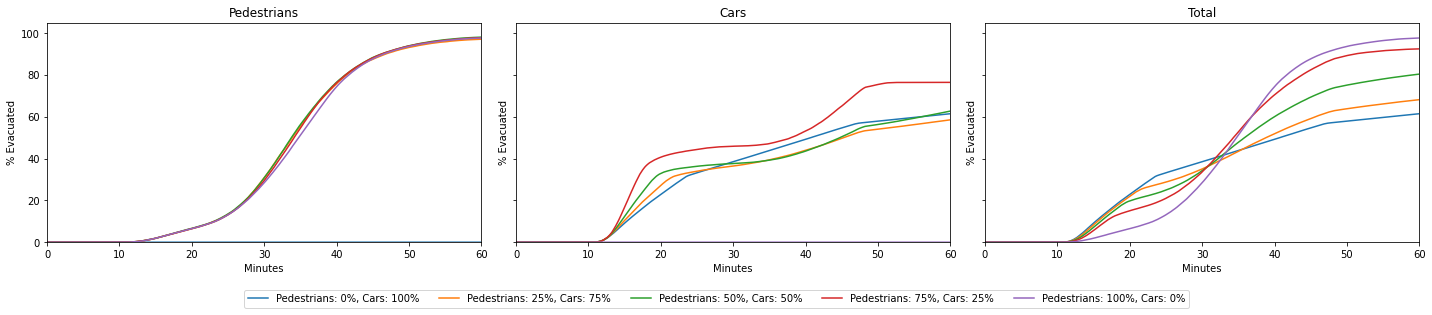
\includegraphics[width=\textwidth]{images/analisi/new-evacuated.png}
    \caption{Percentuale degli evacuati nel tempo al variare del numero di agenti con il modello esteso.}
    \label{fig:analisi-new-evacuated}
\end{figure}

% TODO: riscrivere
Anche per le percentuali di morti figura \ref{fig:analisi-new-casualties} analisi simili alle percentuali di evacuati \ref*{fig:analisi-new-evacuated} possono essere fatte.
%
Si può vedere come al variare del numero di pedoni considerati non ci siano differenze significative,
mentre per le auto la percentuale di vittime sale al crescere del numero di auto considerate.
% TODO: ripetizioni
Il caso con una probabilità di auto del 75\% risulta in una percentuale maggiore di vittime rispetto al caso solo auto.
In generale la percentuale di vittime per le auto è molto più alta rispetto a quella dei pedoni, con un massimo di circa X\% nel caso con una probabilità di auto del 75\%. 
%
Il numero di vittime totali cresce al crescere del numero di auto e il caso con solo auto è quello con la percentuale di mortalità maggiore.

\begin{figure}[ht]
    \centering
    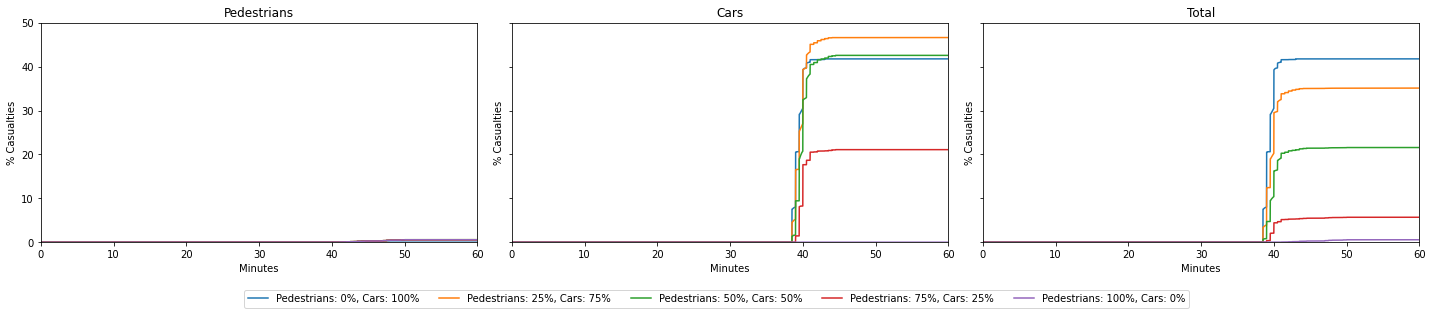
\includegraphics[width=\textwidth]{images/analisi/new-casualties.png}
    \caption{Percentuale delle vittime nel tempo al variare del numero di agenti con il modello esteso.}
    \label{fig:analisi-new-casualties}
\end{figure}

\pagebreak

Nella figura \ref{fig:analisi-new-evtimes} vengono riportate le percentuali di agenti evacuati nel tempo
e il tempo in cui evacuano in media.
%
In modo analogo al modello base il tempo medio di evacuazione si abbassa e sembrano formarsi due picchi nel caso con una probabilità di auto del 25\% per poi appiattirsi
all'aumentare del numero di auto.


\begin{figure}
    \centering
    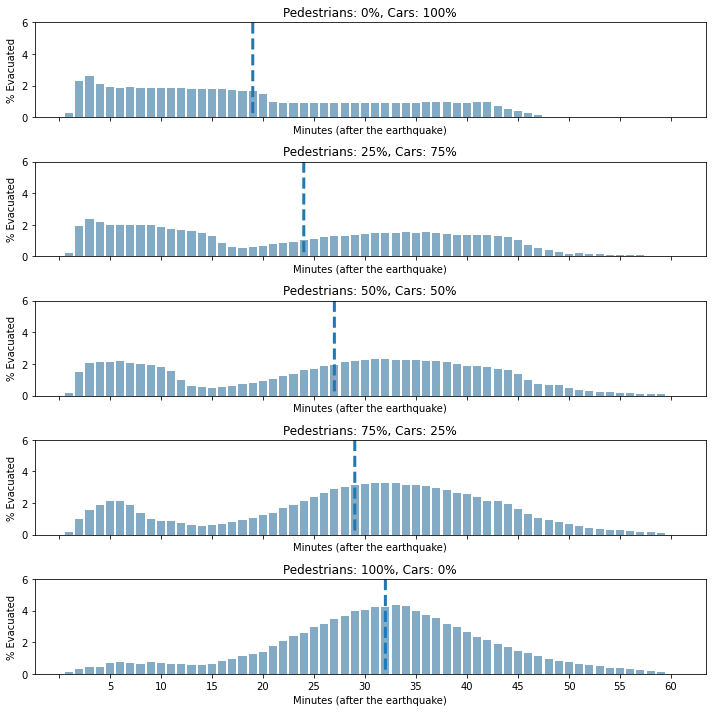
\includegraphics[width=\textwidth]{images/analisi/new-evtimes.png}
    \caption{Distribuzione del tempo di evacuzione in percentuale al variare del numero di agenti e tempo medio di evacuazione.}
    \label{fig:analisi-new-evtimes}
\end{figure}

\pagebreak

\subsection{Comparazione Modello Base e Modello Esteso}
% TODO: sistemare
In questa sottosezione verrano comparati il modello base e il modello esteso analizzando
le percentuali di evacuati e di vittime per poi passare a comparazioni spaziali,
in particolare mostrando l'effetto della gestione delle intersezioni durante la simulazione.

\subsubsection*{Percentuale di Evacuati e di Vittime}

\begin{figure}[ht]
    \centering
    \begin{subfigure}{0.45\textwidth}
        \centering
        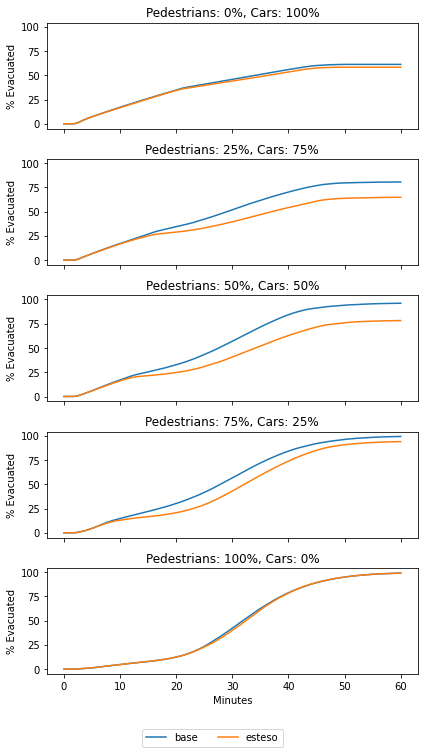
\includegraphics[width=\textwidth]{images/analisi/comparison-total-evacuated.png}
    \end{subfigure}
    \hfill
    \begin{subfigure}{0.45\textwidth}
        \centering
        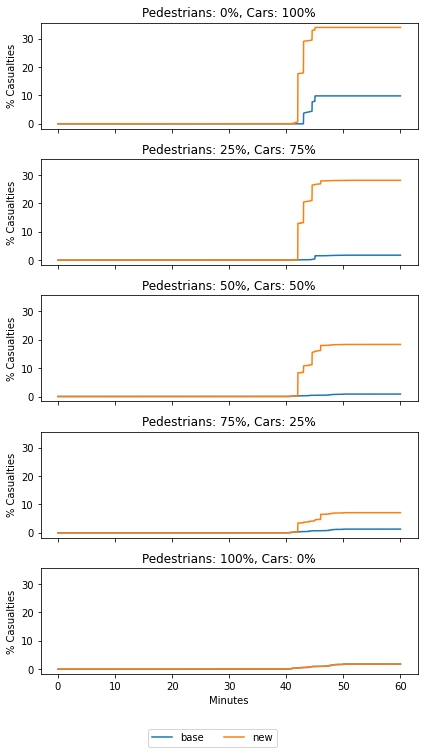
\includegraphics[width=\textwidth]{images/analisi/comparison-total-casualties.png}
    \end{subfigure}
    \caption{Comparazione tra modello base e modello esteso delle percentuali di evacuati (sinistra) e di vittime (destra) al variare del numero di agenti.}
    \label{fig:analisi-comparison-total-ec}
\end{figure}

Osservando la figura \ref{fig:analisi-comparison-total-ec} è possibile comparare le percentuali di evacuati e di vittime nel tempo al variare del numero di agenti tra i due modelli.
In generale il modello esteso presenta un numero minore di evacuati e un numero maggiore di vittime rispetto al modello base.
Questo può essere sintomo dell'effetto delle intersezioni che creando rallentamenti causano una mortalità maggiore,
infatti la percentuale di evacuati del modello esteso presenta un andamento più lento rispetto al modello di partenza.
Per entrambi i modelli la percentuale di evacuati decresce e la percentuale di vittime cresce all'aumentare del numero di auto considerate.
Inoltre per entrambi i modelli le prime vittime si verificano dopo 40 min.
Gli unici casi in cui il modello esteso e quello base hanno risultati molto simili sono il caso con solo pedoni e il caso solo auto, 
ovvero i casi in cui l'effetto delle intersezioni è minimo.

\pagebreak

\subsubsection*{Percentuale di Evacuati nel Tempo}

Come già detto in precedenza le distribuzioni della percentuale di evacuati nel tempo del modello base e del modello esteso 
presentano un andamento simile (Fig. \ref{fig:analisi-comparison-evtimes}). Il tempo medio di evacuazione abbastanza simile per i due modelli,
leggermente più alto per il modello esteso con una probabilità di pedoni di 75\%.

\begin{figure}[ht]
    \centering
    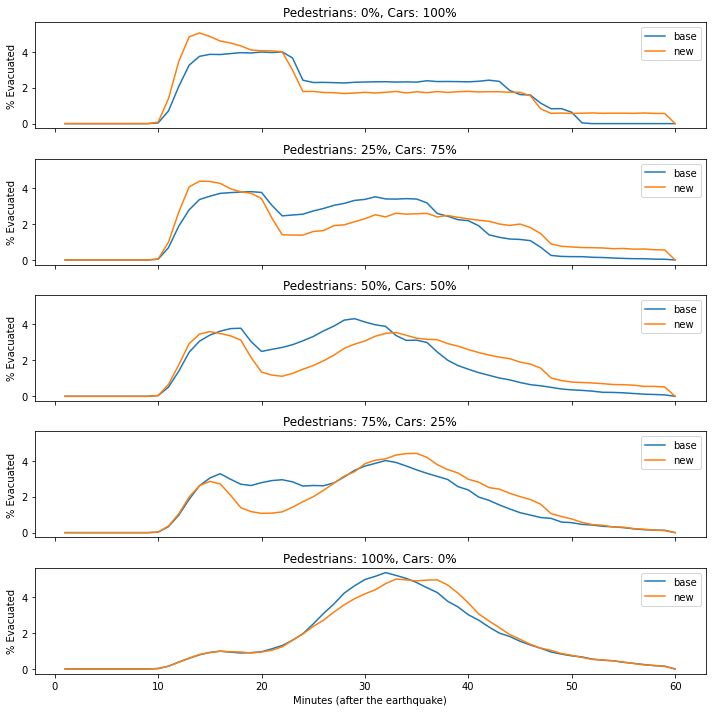
\includegraphics[width=0.9\textwidth]{images/analisi/comparison-evtimes.png}
    \caption{Comparazione delle distribuzioni dei tempi di evacuazione al variare del numero di agenti.}
    \label{fig:analisi-comparison-evtimes}
\end{figure}

\pagebreak

\subsubsection*{Tempo Impiegato per Evacuare}
Un' ulteriore comparazione riguarda il tempo impiegano auto e pedoni per evacuare.
Come mostrato nella figura \ref{fig:analisi-comparison-evtimes2} per quanto riguarda le auto, il modello base presenta un andamento descresente per il tempo medio richiesto per evacuare al diminuire del numero di auto considerate.
Le auto impiegano in media tempi maggiori con il modello esteso rispetto a quello base.
%
I pedoni invece non presentano alcun cambiamento significativo al variare del numero di agenti e del modello considerato. 

Per entrambi i modelli un pedone impiega in media un tempo di 21 minuti per evacuare e un massimo di 36 minuti.
Per le auto invece il tempo medio di evacuazione per il modello base è 10 minuti e per il modello esteso 16 minuti, 
con tempi massimi rispettivamente di 32 e 42 minuti.

\begin{figure}[ht]
    \centering
    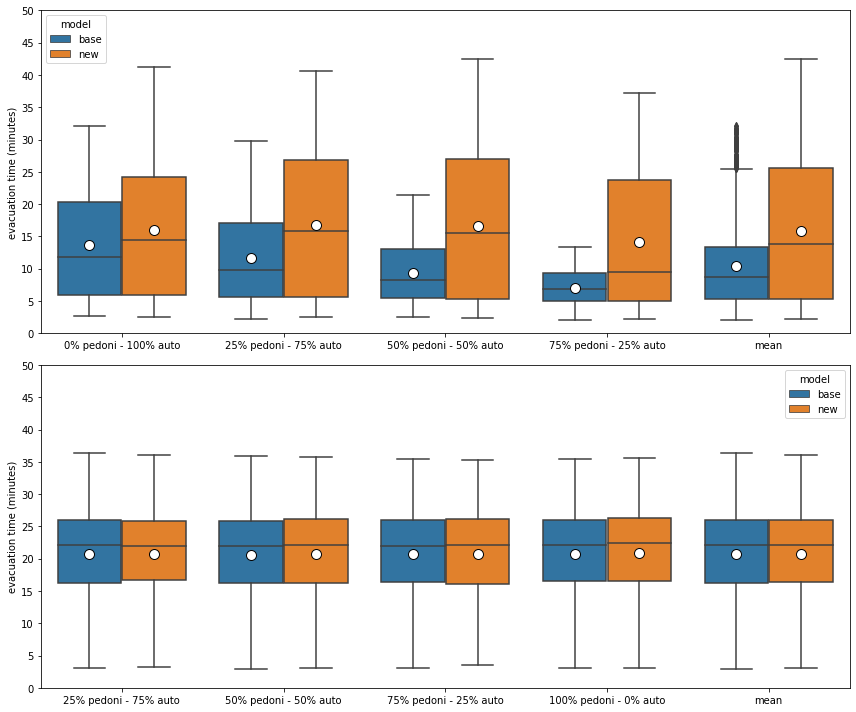
\includegraphics[width=\textwidth]{images/analisi/comparison-evtimes2.png}
    \caption{
        Comparazione dei tempi di evacuazione al variare del numero di agenti e nel caso medio distinti per auto (sopra) e pedoni (sotto).
    }
    \label{fig:analisi-comparison-evtimes2}
\end{figure}

\pagebreak

La figura \ref{fig:analisi-comparison-ev-times-map} mostra i tempi di evacuazione mediati tra gli agenti che partono dalla stessa intersezione,
mediati a loro volta tra tutte le configurazioni di auto e pedoni.

In generale gli agenti che partono dalla costa impiegano più tempo rispetto agli altri che sono più vicini ai rifugi.

Confrontando i pedoni al variare del modello usato non si riscontrano cambiamenti significativi nei tempi di evacuazione.
Mentre nel caso delle auto si nota che il modello esteso introduca dei rallentamenti rispetto al modello base, soprattuto lungo la costa.

\begin{figure}[ht]
    \centering
    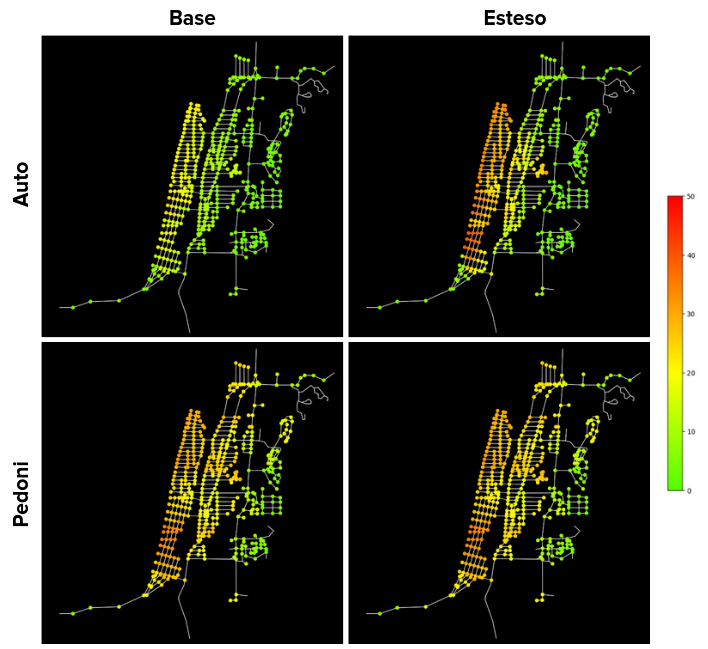
\includegraphics[width=0.8\textwidth]{images/analisi/comparison-evtimes-map.png}
    \caption{Comparazione dei tempi di evacuazione mediati tra gli agenti che partono dalla stessa intersezione. }
    \label{fig:analisi-comparison-ev-times-map}
\end{figure}

\pagebreak

\subsubsection*{Strade Critiche}
Un'ulteriore analisi per valutare l'effetto dell'estensione del modello è quella di evidenziare in quali strade si verificano 
più vittime al variare del numero di auto e pedoni. 
%
Nella figura \ref{fig:analisi-comparison-critical-links1} viene mostrato come si distribuisce la percentuale di mortalità nelle strade 
al variare del numero di auto e pedoni e riportata la percentuale media. 

Il modello base (Fig. \ref{fig:base-link-casualties}) nei casi con un numero di auto minore o uguale al 50\%
non presenta differenze significative e si hanno tante strade con una percentuale bassa di vittime, 
mentre negli altri due casi ci sono poche strade con una percentuale alta.

Il modello esteso (Fig. \ref{fig:new-link-casualties}) invece presenta una strada comune per tutti casi 
in cui sono presenti delle auto che contribuisce a più del 50\% delle vittime.
%
In generale in tutti i casi la maggior parte delle strade con più vittime sono diverse tra i due modelli a eccezione del caso 
100\% pedoni.
%
Le strade segnate come critiche corrispondono a quelle con una percentuale media maggiore del 5\% e sono mostrate nella figura \ref{fig:analisi-comparison-critical-links2}.

\begin{figure}[ht]
    \centering
    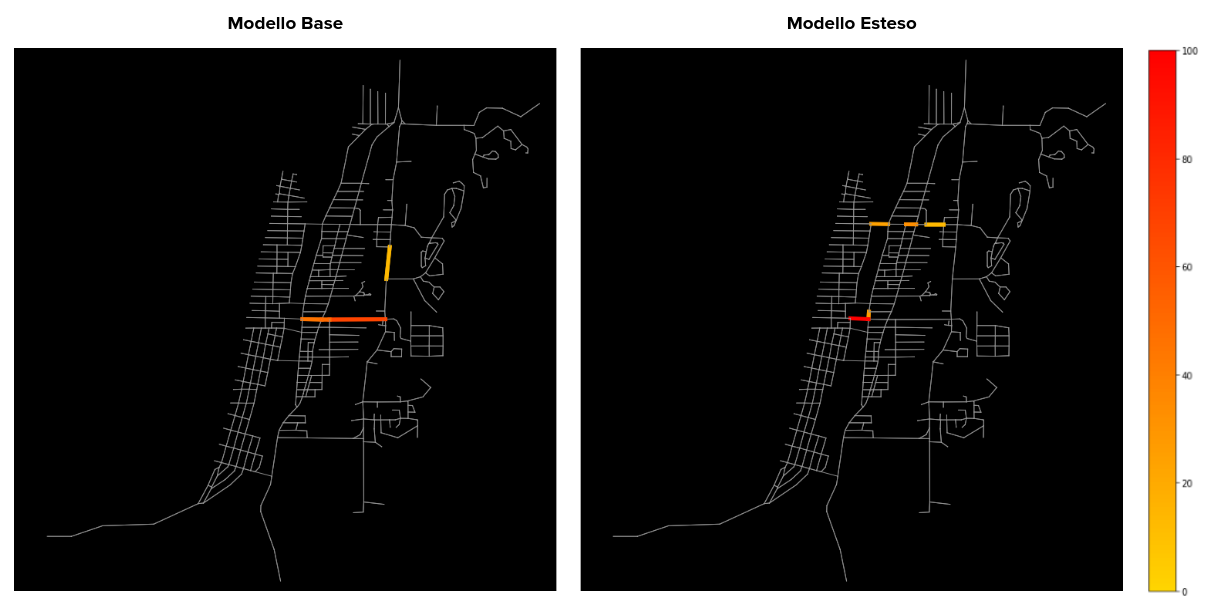
\includegraphics[width=0.8\textwidth]{images/analisi/casualties-map.png}
    \caption{strade critiche trovate per i due modelli.}
    \label{fig:analisi-comparison-critical-links2}
\end{figure}

\newpage

\begin{figure}[ht]
    \centering
    \begin{subfigure}{0.475\textwidth}
        \centering
        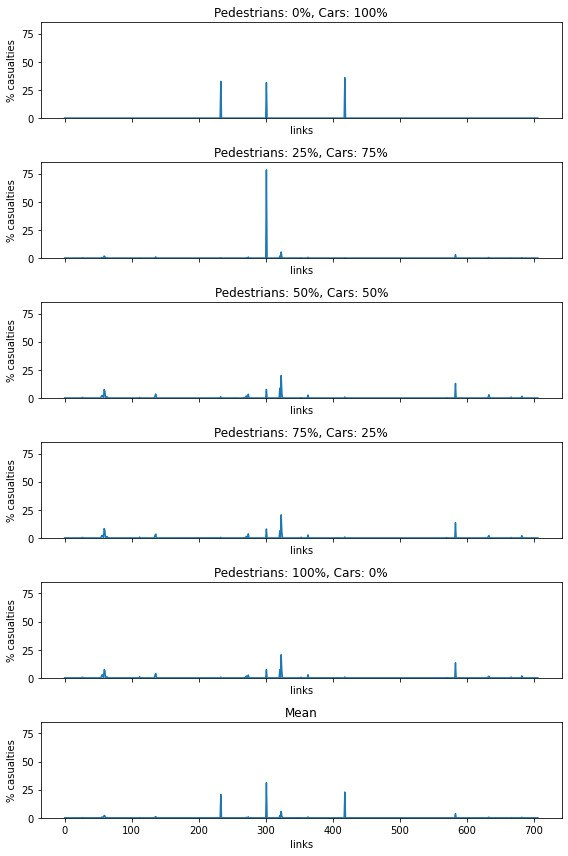
\includegraphics[width=\textwidth]{images/analisi/base_links_casualties}
        \caption{Modello base}
        \label{fig:base-link-casualties}
    \end{subfigure}
    \hfill
    \begin{subfigure}{0.475\textwidth}
        \centering
        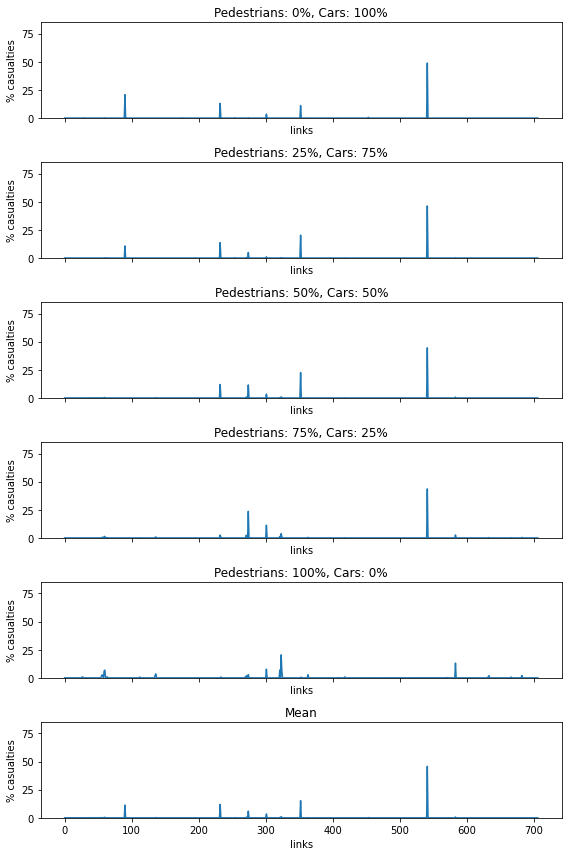
\includegraphics[width=\textwidth]{images/analisi/new_links_casualties}
        \caption{Modello esteso}
        \label{fig:new-link-casualties}
    \end{subfigure}
    \caption{Comparazione delle percentuali di mortalità nelle strade al variare del numero di auto e pedoni.}
    \label{fig:analisi-comparison-critical-links1}
\end{figure}


\newpage

\subsection{Analisi Intersezioni}
In questa sottosezione verranno descritte le analisi effettuate sulle intersezioni per valutare l'effetto dell'estesione 
del modello. Sono state identificate le intersezioni critiche, ovvero quelle con un alta mortalità. Successivamente 
sono stati analizzati il flusso in entrata e in uscita e i tempi di attesa delle intersezioni, evidenziando le differenze tra le 
intersezioni critiche e non critiche.

\subsubsection*{Intersezioni Critiche}
Per identificare le intersezioni critiche (Fig. \ref{fig:analisi-comparison-critical-ints2}) è stato considerato il numero totale di vittime delle strade 
in entrata di ogni intersezione e sono state selezionate quelle con una percentuale di vittime superiore o uguale al 5\%.

Come effettuato per le strade critiche (Fig. \ref{fig:analisi-comparison-critical-links1}), il numero di vittime considerato è quello mediato al variare del numero di auto e pedoni (Fig. \ref{fig:analisi-comparison-critical-ints1}).

\begin{figure}[ht]
    \centering
    \begin{subfigure}{0.45\textwidth}
        \centering
        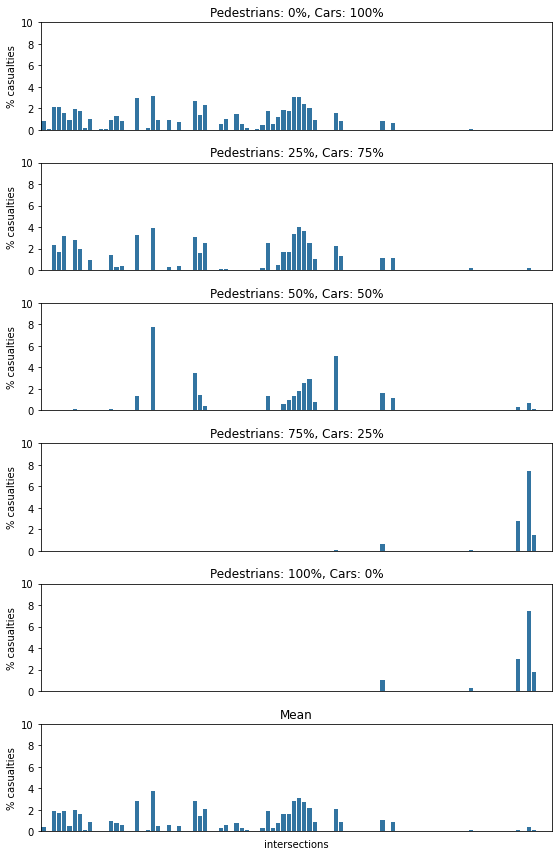
\includegraphics[width=\textwidth]{images/analisi/comparison-critical-ints-base.png}
        \caption{Modello base}
        \label{fig:base-ints-casualties}
    \end{subfigure}
    \hfill
    \begin{subfigure}{0.45\textwidth}
        \centering
        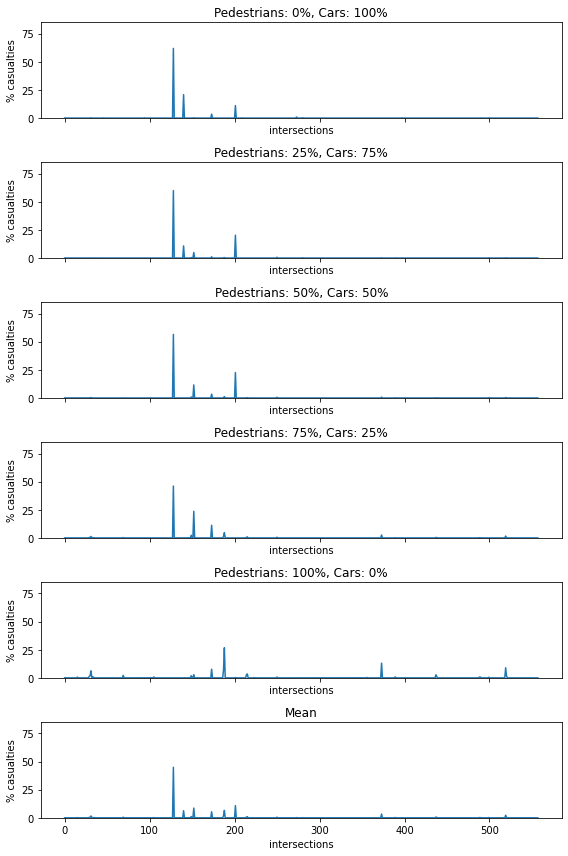
\includegraphics[width=\textwidth]{images/analisi/comparison-critical-ints-new.png}
        \caption{Modello esteso}
        \label{fig:new-ints-casualties}
    \end{subfigure}
    \caption{Comparazione delle percentuali di mortalità nelle intersezioni al variare del numero di auto e pedoni.}
    \label{fig:analisi-comparison-critical-ints1}
\end{figure}

\pagebreak

Nella figura \ref{fig:analisi-comparison-critical-ints2} vengono mostrate le intersezioni identificate 
come critiche e distinte in base al tipo di intersezione: TWSC, AWSC e incroci con 3 strade.

Alcune delle intersezioni critiche sono in comune tra i due modelli, tuttavia contribuiscono in modo diverso al totale di vittime.
Nel modello base la percentuale maggiore di vittime si trova più vicino ai rifugi rispetto al modello esteso in cui la percentuale maggiore si trova nel centro.

\begin{figure}[ht]
    \centering
    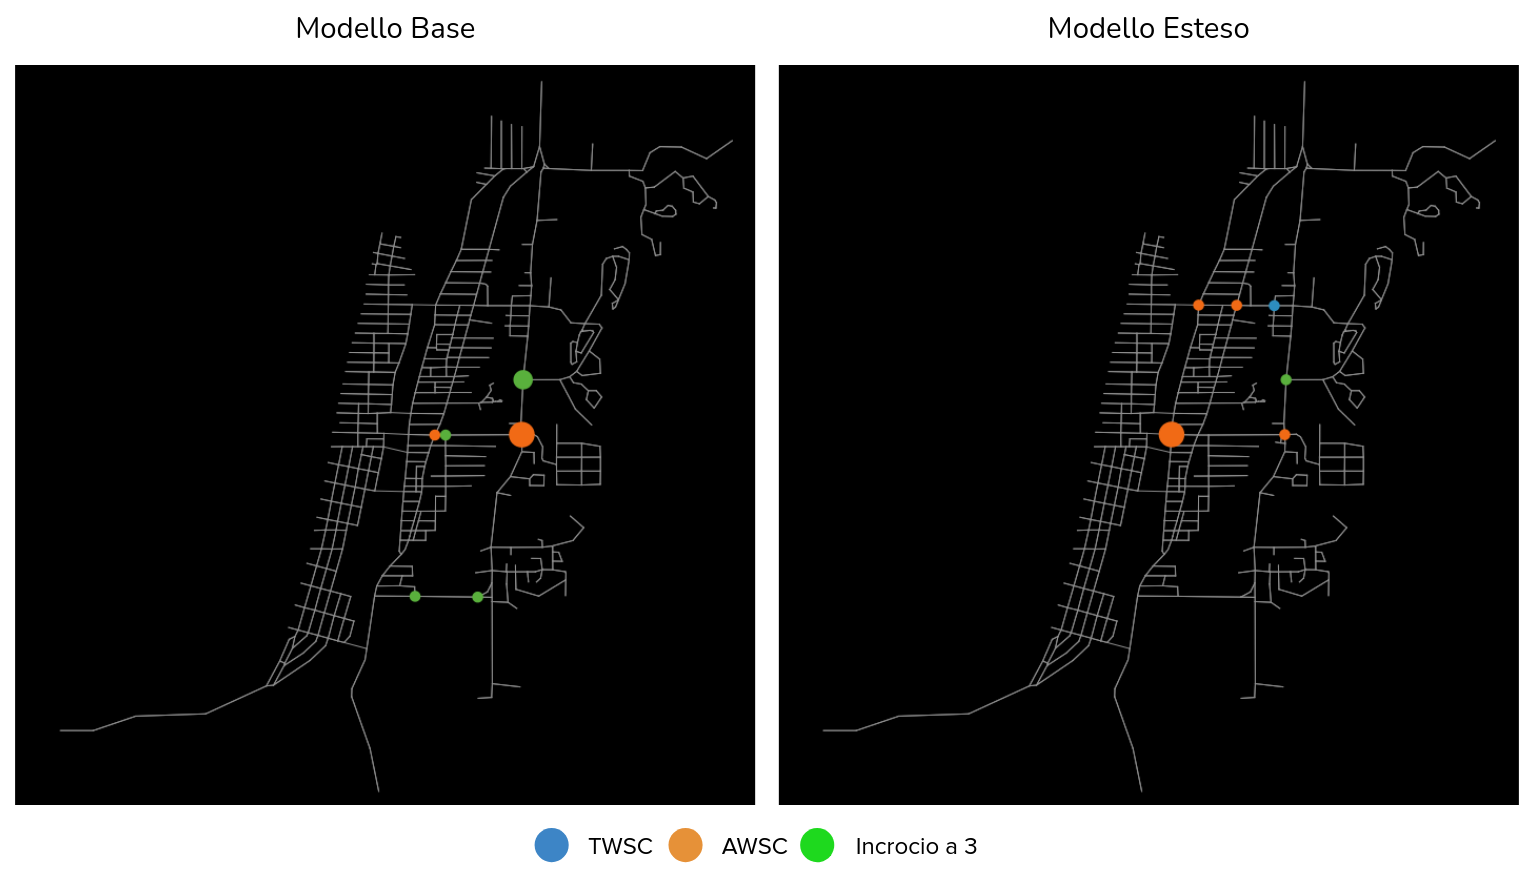
\includegraphics[width=0.8\textwidth]{images/analisi/critical_ints_map.png}
    \caption{Intersezioni critiche distinte per tipo di intersezione. La dimensione dei punti indica la percentuale di vittime delle strade in entrata.}
    \label{fig:analisi-comparison-critical-ints2}
\end{figure}


\subsubsection*{Flusso}
Per ogni intersezione è stato calcolato il flusso in entrata e in uscita sommando i valori di ogni strada al variare del numero di auto e pedoni.

Come si nota nella figura \ref{fig:analisi-comparison-in-out-flow-ped}, 
il flusso dei pedoni non presenta particolari differenze tra modello base ed esteso, nonostante le modifiche apportate ai pedoni.

Per entrambi i modelli il flusso in entrata e in uscita in ogni intersezione è molto simile.
Inoltre all'aumentare del numero di pedoni c'è un incremento nel flusso.

Nella maggior parte dei casi il flusso delle intersezioni TWSC risulta più basso rispetto a quelle AWSC, poichè la strada secondaria 
è bloccata finchè la principale è occupata.

\begin{figure}[p]
    \centering
    \begin{subfigure}{\textwidth}
        \centering
        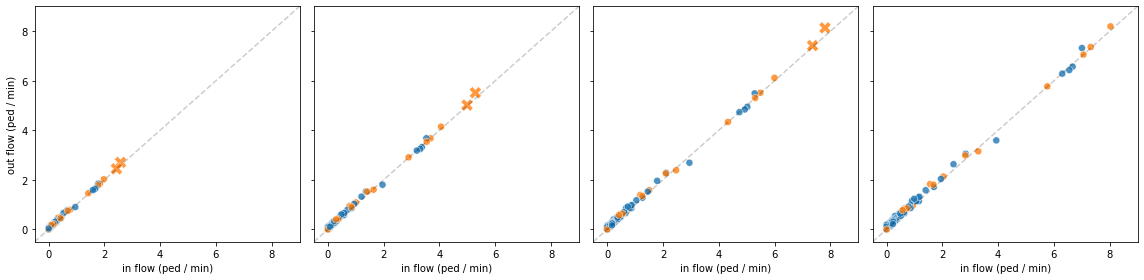
\includegraphics[width=\textwidth]{images/analisi/comparison-base-in-out-flow-ped.png}
        \caption{Modello base}
    \end{subfigure}
    
    \begin{subfigure}{\textwidth}
        \centering
        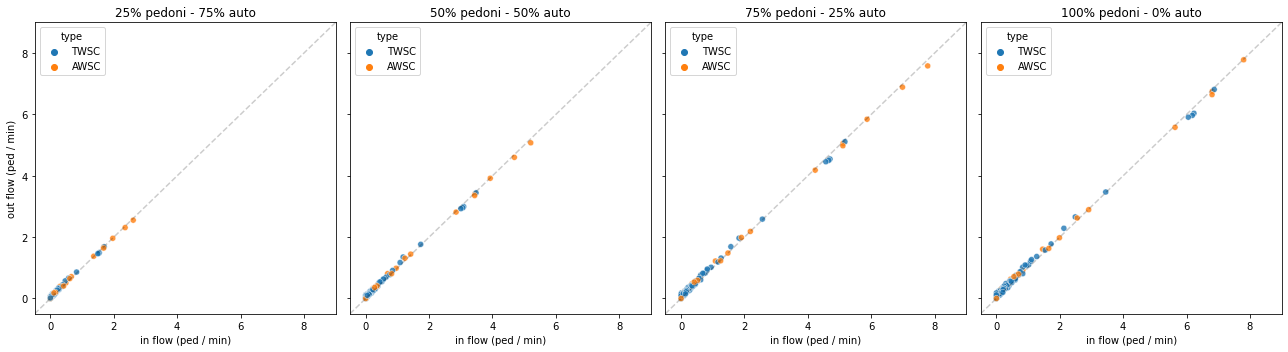
\includegraphics[width=\textwidth]{images/analisi/comparison-new-in-out-flow-ped.png}
        \caption{Modello esteso}
    \end{subfigure}
    \caption{
        Confronto tra il flusso dei pedoni in entrata e in uscita per ogni intersezione al variare del numero di auto e pedoni.
    }
    \label{fig:analisi-comparison-in-out-flow-ped}
\end{figure}

Osservando il flusso delle auto (Fig. \ref{fig:analisi-comparison-in-out-flow-car}) 
viene sempre riscontrato un incremento di flusso all'aumentare del numero di auto.

In questo caso però il flusso in entrata e in uscita non sono perfettamente bilanciati e risultano più sparsi rispetto al flusso dei pedoni.
Inoltre il flusso in entrata è quasi sempre maggiore del flusso in uscita.

Nel modello esteso in generale il flusso risulta più basso,
probabilmente a causa della gestione delle intersezioni che, combinato all'utilizzo dello \textit{shortest path}, 
provoca un rallentamento al traffico in uscita che, propagandosi in tutta la rete, abbassa il flusso in tutte le intersezioni.

\begin{figure}[p]
    \centering
    \begin{subfigure}{\textwidth}
        \centering
        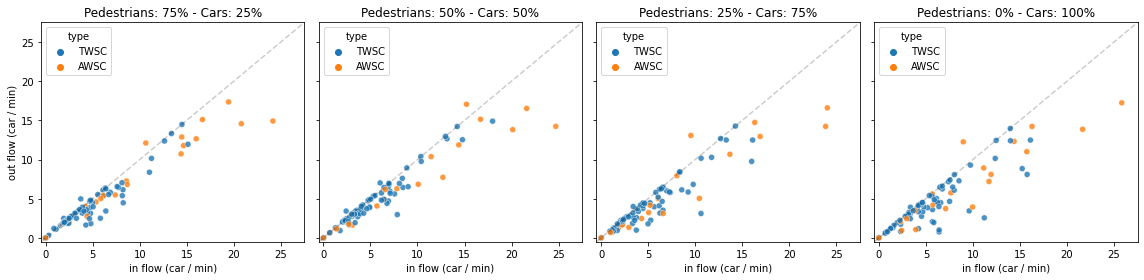
\includegraphics[width=\textwidth]{images/analisi/comparison-base-in-out-flow-car.png}
        \caption{Modello base}
    \end{subfigure}

    \begin{subfigure}{\textwidth}
        \centering
        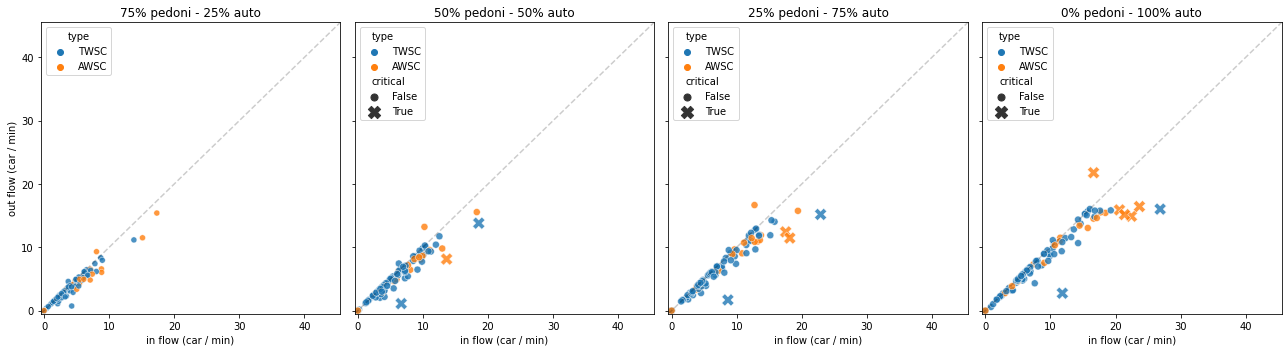
\includegraphics[width=\textwidth]{images/analisi/comparison-new-in-out-flow-car.png}
        \caption{Modello esteso}
    \end{subfigure}
    \caption{
        Confronto tra il flusso delle auto in entrata e in uscita per ogni intersezione al variare del numero di auto e pedoni.
    }
    \label{fig:analisi-comparison-in-out-flow-car}
\end{figure}


\subsubsection*{Tempi di Attesa}

Infine esclusivamente per il modello esteso vengono analizzati i tempi di attesa nelle intersezioni per le auto,
ovvero il tempo che passa da quando un'auto arriva all'incrocio a quando ha il via libera. 
Inoltre i tempi sono distinti tra i due tipi di intersezione: AWSC e TWSC.

Come si può vedere nella tabella \ref{tab:analisi-car-delay}, con una percentuale più bassa di auto le intersezioni AWSC 
hanno in media tempi di attesa più lunghi mentre le intersezioni TWSC hanno tempi più brevi.

Per quanto riguarda le intersezioni TWSC, i tempi di attesa massimi sono più alti rispetto agli AWSC in tutti i casi a eccezione di quello con 25\% auto, 
per via della presenza degli stop nelle strade secondarie.

Nella figura \ref{fig:analisi-comparison-car-delay} vengono riportati i tempi di attesa al variare del numero di auto,
per ogni intersezione.



\begin{table}[ht]
    \centering
    \begin{tabular}{|c|c|c|c|c|c|}
    \hline
         & 25\% cars & 50\% cars & 75\% cars & 100\% cars & intersection \\ \hline
    mean & 34 s  & 32 s  & 29 s  & 24 s  & AWSC         \\ \hline
    max  & 267 s & 184 s & 202 s & 225 s & AWSC         \\ \hline
    mean & 8 s   & 13 s  & 18 s  & 31 s  & TWSC         \\ \hline
    max  & 142 s & 189 s & 237 s & 406 s & TWSC         \\ \hline
    \end{tabular}
    \caption{Confronto dei tempi di attesa massimi e medi per i due tipi di intersezioni al variare della percentuale di auto considerate.}
    \label{tab:analisi-car-delay}
\end{table}



\begin{figure}[ht]
    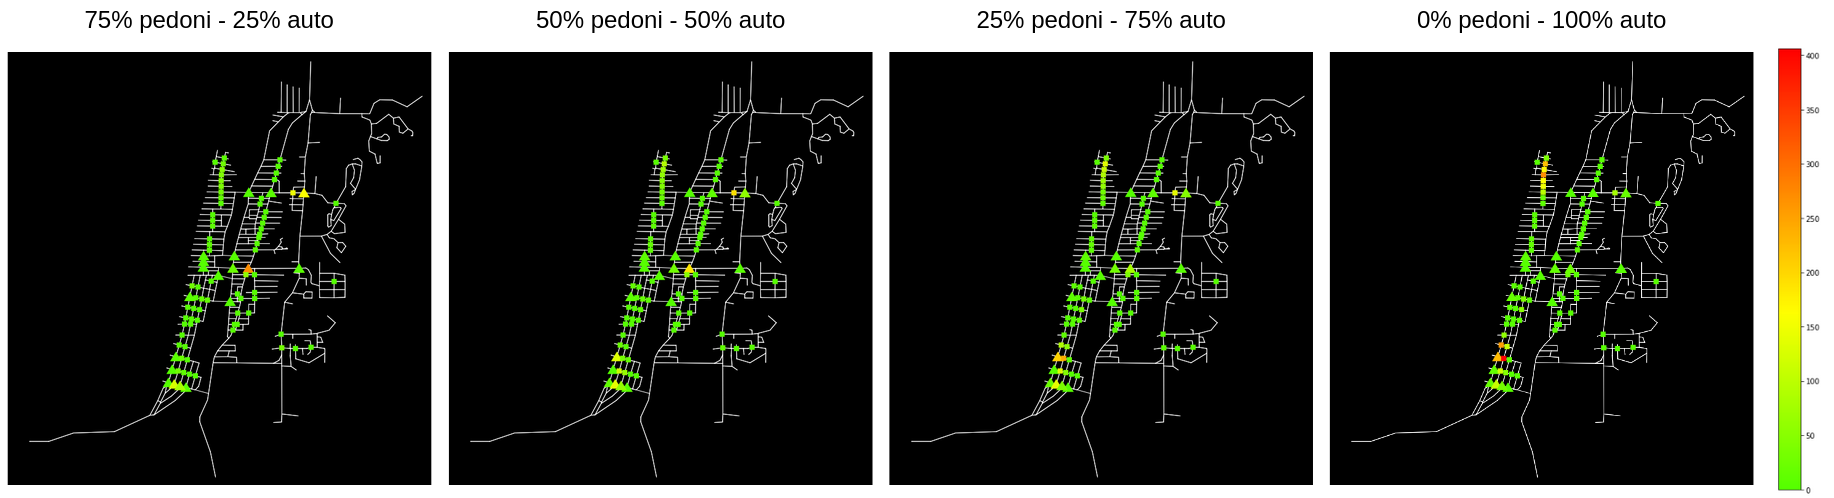
\includegraphics[width=1\textwidth]{images/analisi/comparison-car-delay.png}   
    \caption{tempi di attesa nelle intersezioni al variare del numero di auto, differenziando AWSC (triangoli) e TWSC (cerchi).}
    \label{fig:analisi-comparison-car-delay}
\end{figure}

\begin{figure}[ht]
    \centering
    \begin{subfigure}{0.75\textwidth}
        \centering
        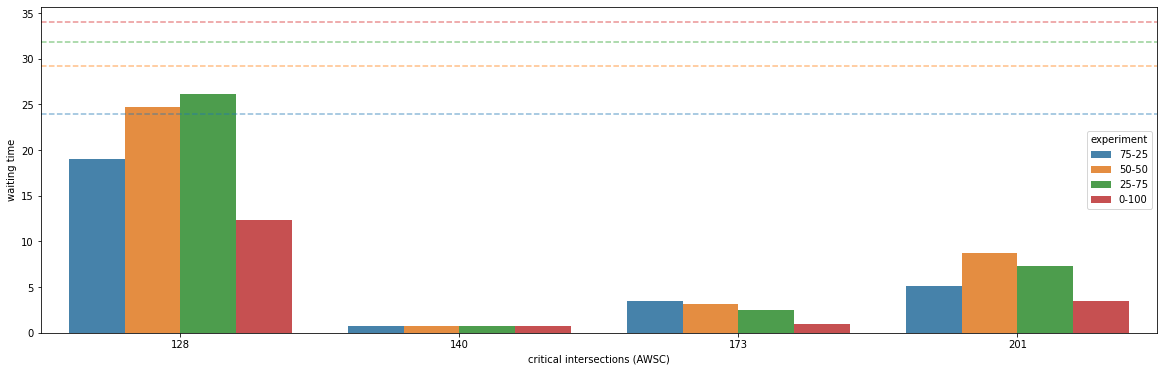
\includegraphics[width=\textwidth]{images/analisi/critical_waiting_time_awsc.png}
        \caption{AWSC}
        \label{fig:critical-waiting-times-awsc}
    \end{subfigure}
    \hfill
    \begin{subfigure}{0.175\textwidth}
        \centering
        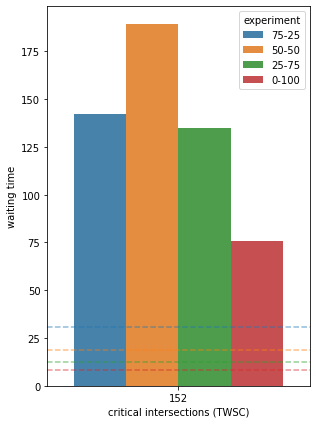
\includegraphics[width=\textwidth]{images/analisi/critical_waiting_time_twsc.png}
        \caption{TWSC}
        \label{fig:critical-waiting-times-twsc}
    \end{subfigure}
    \caption{comparazione tempi di attesa delle intersezioni critiche di tipo AWSC (a) e TWSC (b) rispetto a tutte le intersezioni al variare del numero di auto.}
    \label{fig:critical-waiting-times}
\end{figure}

\newpage

\subsection*{Comparazione Modello Base con Modello Wang 2021}


\section{Conclusioni}
\label{sec:conclusione}
% In questo lavoro è stato implementato un modello agent-based per la simulazione di evacuazione in caso di tsunami.
% Il modello di \textcite{wang2016agent} è stato usato come base di partenza ed esteso aggiungendo una velocità 
% dinamica ai pedoni e la gestione delle interazioni tra auto e pedoni.

% Successivamente sono stati effettuati diversi esperimenti al variare del numero di auto e pedoni.
% I risultati di ogni esperimento sono stati mediati tra 30 simulazioni per via della randomicità di alcuni parametri 
% e sono stati confrontati con il modello di partenza e in seguito con il modello di \textcite{wang2021novel}. 

% I risultati ottenuti sono meno ottimistici rispetto al modello base.  
% La gestione delle intersezioni aumenta la mortalità e i tempi medi di evacuazione delle auto.
% In generale i tempi di attesa nelle intersezioni aumentano al crescere del numero di auto e sono più alti nelle intersezioni di tipo TWSC.
% %
% L'aggiunta della velocità dinamica per i pedoni non ha un grosso impatto nell'evacuazione in quanto 
% i pedoni non raggiungono ....
% %
% Il caso in cui riescono a evacuare più agenti è quello con soli pedoni.

In questo lavoro è stato implementato un modello agent-based per la simulazione di evacuazione in caso di tsunami.
Il modello di \textcite{wang2016agent} è stato usato come base di partenza ed esteso aggiungendo una velocità 
dinamica ai pedoni e la gestione delle interazioni tra auto e pedoni in particolare nelle intersezioni.

Successivamente sono stati effettuati diversi esperimenti al variare del numero di auto e pedoni.
I risultati di ogni esperimento sono stati mediati tra 30 simulazioni per via della randomicità di alcuni parametri 
e sono stati confrontati con il modello di partenza e in seguito con il modello di \textcite{wang2021novel}.

Comparato al modello base il modello esteso ha risultati meno ottimistici.
La gestione delle intersezioni rallenta l'evacuazione poichè aggiunge dei tempi di attesa nelle intersezioni,
abbassa il flusso sia in entrata che in uscita e di conseguenza si ha un numero minore di evacuati e 
un numero maggiore di vittime rispetto al modello base, soprattutto nei casi con più auto.

In generale i tempi di attesa nelle intersezioni aumentano al crescere del numero di auto e sono più alti nelle intersezioni di tipo TWSC.

Per quanto riguarda i pedoni non sembra esserci alcun cambiamento significativo,
infatti si hanno delle percentuali di vittime, evacuati e tempi di evacuazione molto simili con il modello base.

Il numero di evacuati aumenta al diminuire del numero di auto, quindi il caso migliore risulta essere quello con solo pedoni.
Infatti come suggerito dal piano di evacuazione della città di Seaside\footnote{\url{https://www.oregongeology.org/pubs/tsubrochures/SeasideGearhart-EvacBrochure_onscreen.pdf}}
la modalità di evacuazione consigliata è quella a piedi.

Le intersezioni con una mortalità maggiore corrispondono a  
intersezioni con un flusso in entrata basso, un tempo di attesa alto e che sono situate vicino alla costa.

Infine comparato al modello di \textcite{wang2021novel} il modello base e il modello esteso presentano un numero significativamente maggiore di evacuati e un numero minore di vittime, soprattuto per le auto.

Per i pedoni, nonostante le differenze nel numero di agenti, larghezza della strada e tempi di partenza, è riscontrabile qualche similitudine. 
La differenza maggiore tra i modelli è nelle vittime che per il modello di \textcite{wang2021novel} si verficano gradualmente tra il minuto 28 e il minuto 50, mentre nel modello
base e nel modello esteso si verficano in poco tempo vicino a 40 minuti.
In particolare il modello esteso risulta più ottimistico per evacuati e vittime rispetto al modello di \textcite{wang2021novel} nonostante la gestione delle intersezioni 
che prevede un rallentamento del traffico e più vittime rispetto al modello base.

\subsection{Sviluppi Futuri}
Diverse sono le limitazioni riguardanti la gestione delle intersezioni, per i pedoni non viene gestito alcun coordinamento pedone-pedone nelle intersezioni, inoltre
potrebbero essere implementate delle attese anche per i pedoni nel caso delle auto stiano attraversando.

% TODO: fix
Un'altra limitazione è l'utilizzo del percorso più breve, altre strategie di \textit{routing} più realistiche potrebbero essere usate come ad esempio Nash equilibrium.
Per i percorsi dei pedoni inoltre si potrebbe creare un secondo grafo per ottimizzare i percorsi tramite i marciapiedi.

In questo lavoro ci si è limitati a intersezioni a 4 strade, esclusivamente di tipo AWSC e TWSC, quindi potrebbero essere considerate
ulteriori tipi d'intersezioni come ad esempio quelle con 3 strade oppure quelle regolate da semafori.

Nelle strade secondarie degli incroci di tipo TWSC si potrebbe usare un raggio di visione che vada oltre la linea di stop
per stabire meglio la presenza di auto nella via principale.

Un'altra possibile aggiunta è quella di introdurre una fase di decelerazione prima di raggiungere la zona di crossing e una fase 
di accelerazione quando si ottiene il via libera.

Ulteriori sviluppi futuri potrebbero concentrarsi sulla validazione del modello. 
Per quanto riguarda la gestione delle intersezioni si potrebbe usare il modello HCM \parencite{transportation2000highway} 
per comparare il V/C ratio e delay nelle intersezioni rispetto ai valori del piano stradale di Seaside, Oregon \parencite{seaside2010tsp}.


\pagebreak
\printbibliography

\end{document}
